% Classroom-report LaTeX version, adjusted to match the HW00 indented sample.
\documentclass[12pt,a4paper,fontset=none]{ctexart}

\usepackage[left=2.7cm,right=2.7cm,top=2.5cm,bottom=2.5cm]{geometry}
\usepackage{amsmath, amssymb}
\usepackage{booktabs}
\usepackage{longtable}
\usepackage{array}
\usepackage{calc}
\usepackage[font=small,labelfont=bf,labelsep=quad]{caption}
\usepackage{graphicx}
\usepackage{float}
\usepackage{hyperref}
\usepackage{xurl}
\usepackage{xcolor}
\usepackage{fancyvrb}
\usepackage{fvextra}
\usepackage{setspace}
\usepackage{enumitem}
\usepackage{etoolbox}

\let\OriginalIncludeGraphics\includegraphics
\renewcommand{\includegraphics}[2][]{%
  \OriginalIncludeGraphics[width=\linewidth,height=0.88\textheight,keepaspectratio,#1]{#2}%
}

\setmainfont{Noto Serif CJK SC}
\setCJKmainfont{Noto Serif CJK SC}
\setmonofont[Scale=0.9]{DejaVu Sans Mono}
\setCJKmonofont[Scale=0.9]{Noto Sans CJK SC}
\renewcommand{\texttt}[1]{{\ttfamily\footnotesize #1}}
\graphicspath{{../}{../assets/}{../../../result/}{../../../results/}{../../../outputs/}}
\setstretch{1.36}
\AtBeginDocument{\zihao{-4}\selectfont}
\setlength{\parindent}{2em}
\setlength{\parskip}{0pt}
\setlength{\abovedisplayskip}{0.65\baselineskip}
\setlength{\belowdisplayskip}{0.65\baselineskip}
\captionsetup{skip=0.35\baselineskip}
\sloppy
\clubpenalty=10000
\widowpenalty=10000

\hypersetup{hidelinks}

\setcounter{secnumdepth}{3}
\setcounter{tocdepth}{2}
\renewcommand{\thesubsection}{\arabic{subsection}}
\renewcommand{\thesubsubsection}{\thesubsection.\arabic{subsubsection}}
\ctexset{
  section = {
    format = {\centering\zihao{4}\bfseries},
    aftername = {\quad},
    beforeskip = {1.1\baselineskip},
    afterskip = {0.65\baselineskip}
  },
  subsection = {
    format = {\zihao{-3}\bfseries},
    aftername = {\quad},
    beforeskip = {1.0\baselineskip},
    afterskip = {0.45\baselineskip}
  },
  subsubsection = {
    format = {\zihao{4}\bfseries},
    aftername = {\quad},
    beforeskip = {0.75\baselineskip},
    afterskip = {0.25\baselineskip}
  }
}

\DefineVerbatimEnvironment{verbatim}{Verbatim}{
  fontsize=\footnotesize,
  frame=single,
  framesep=0.5em,
  xleftmargin=1.2em,
  xrightmargin=1.2em,
  breaklines=true,
  breakanywhere=true
}
\providecommand{\tightlist}{\setlength{\itemsep}{0pt}\setlength{\parskip}{0pt}}
\providecommand{\pandocbounded}[1]{#1}
\newcounter{none}
\newcommand{\passthrough}[1]{#1}
\setlist{nosep,leftmargin=2em}
\setlength{\LTpre}{0.35\baselineskip}
\setlength{\LTpost}{0.35\baselineskip}
\newif\ifwidetable
\newif\iftighttable
\setlength{\tabcolsep}{4pt}
\AtBeginEnvironment{longtable}{%
  \iftighttable
    \small\setlength{\tabcolsep}{1pt}%
  \else\ifwidetable
    \footnotesize\setlength{\tabcolsep}{2pt}%
  \else
    \normalsize\setlength{\tabcolsep}{4pt}%
  \fi\fi
  \renewcommand{\arraystretch}{1.16}%
  \renewcommand{\texttt}[1]{{\ttfamily #1}}%
}
\emergencystretch=3em
\newcommand{\fileinline}[1]{{\urlstyle{same}\nolinkurl{#1}}}
\newcommand{\metadataline}[1]{#1}
\newcommand{\scriptpath}[1]{\fileinline{#1}}
\newcommand{\githubscriptsbase}{https://github.com/Void0312Aurora/computational-physics-homework-2026/blob/main/07/scripts}
\newcommand{\scriptlink}[1]{\noindent\metadataline{\textbf{相关脚本：}\href{../../../scripts/#1}{本地 \scriptpath{scripts/#1}} / \href{\githubscriptsbase/#1}{GitHub \scriptpath{scripts/#1}}}\par\medskip}

\title{\vspace{-1.0em}{\bfseries\zihao{3} HW08 小组作业报告}\\[0.35em]{\zihao{-4} 数值积分方法实验报告：段首缩进版}}
\author{\zihao{-4} 姜玥晟、周鑫志、高西飞}
\date{\zihao{-4} 2026-04-29}

\begin{document}
\pagestyle{plain}
\maketitle

\begin{figure}[H]
  \centering
  \begin{minipage}[t]{0.27\linewidth}
    \centering
    
\includegraphics[width=0.82\linewidth]{pic_1.jpg}\\[0.35em]
    姜玥晟
  \end{minipage}
  \hspace{0.04\linewidth}
  \begin{minipage}[t]{0.27\linewidth}
    \centering
    
\includegraphics[width=0.82\linewidth]{pic_2.jpg}\\[0.35em]
    周鑫志
  \end{minipage}
  \hspace{0.04\linewidth}
  \begin{minipage}[t]{0.27\linewidth}
    \centering
    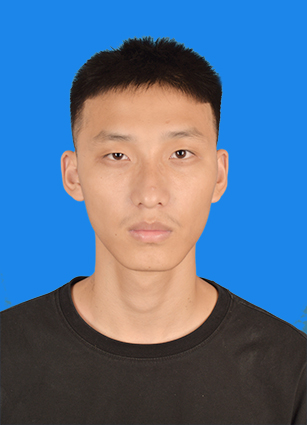
\includegraphics[width=0.82\linewidth]{pic_3.jpg}\\[0.35em]
    高西飞
  \end{minipage}
\end{figure}

\begin{table}[H]
  \centering
  \begin{tabular}{ll}
    \toprule
    项目 & 内容 \\
    \midrule
    源题编号 & HW08 \\
    作业属性 & 小组作业 \\
    小组成员 & 姜玥晟、周鑫志、高西飞 \\
    报告主题 & Simpson 积分、自适应积分、Romberg 外推、变量代换与超球体积 \\
    实验环境 & Python 3.13.5、numpy、matplotlib \\
    \bottomrule
  \end{tabular}
\end{table}

\newpage
\renewcommand{\contentsname}{目录}
\tableofcontents
\newpage

\section*{I. 固体热容的 Debye 积分}\label{i.-ux56faux4f53ux70edux5bb9ux7684-debye-ux79efux5206}
\addcontentsline{toc}{section}{I. 固体热容的 Debye 积分}

本组问题使用 Debye 固体理论计算固体在温度 \(T\) 下的定容热容

\[
C_V=9V\rho k_B\left(\frac{T}{\theta_D}\right)^3
\int_0^{\theta_D/T}\frac{x^4e^x}{(e^x-1)^2}\,dx.
\]

其中 \(V\) 是固体体积，\(\rho\) 是原子数密度，\(k_B\) 是 Boltzmann 常数，\(\theta_D\) 是 Debye 温度。

\subsection{Problem 1(a)：计算 Debye 热容函数}\label{problem-1a}

\scriptlink{problem1.py}

\subsubsection{待求问题}\label{ux5f85ux6c42ux95eeux9898}

编写函数 \(C_V(T)\)，计算给定温度下的热容。样品为 \(1000\,\mathrm{cm^3}\) 的固体铝，原子数密度为 \(\rho=6.022\times10^{28}\,\mathrm{m^{-3}}\)，Debye 温度为 \(\theta_D=428\,\mathrm{K}\)。使用 Simpson 法计算积分，取 \(N=50\) 个采样区间。

\subsubsection{解决方式}\label{ux89e3ux51b3ux65b9ux5f0f}

样品体积先换算为

\[
V=1000\,\mathrm{cm^3}=10^{-3}\,\mathrm{m^3}.
\]

由于 Simpson 复合公式要求子区间数为偶数，本报告将题面中的 \(N=50\) 作为 \(50\) 个等长子区间。对 \([a,b]\) 上的积分，复合 Simpson 公式为

\[
\int_a^b f(x)\,dx
\approx
\frac{h}{3}\left[f(x_0)+f(x_N)
+4\sum_{j=1,3,\ldots,N-1}f(x_j)
+2\sum_{j=2,4,\ldots,N-2}f(x_j)\right],
\]

其中 \(h=(b-a)/N\)。Debye 被积函数在 \(x=0\) 处为可去奇点，因为

\[
\frac{x^4e^x}{(e^x-1)^2}=x^2-\frac{x^4}{12}+O(x^6),
\]

所以程序在零点附近使用该展开避免出现 \(0/0\)。计算 \(C_V(T)\) 的流程如下：

\begin{verbatim}
Input : temperature T, Simpson slices N = 50
Output: heat capacity C_V(T)

V <- 1000e-6
rho <- 6.022e28
theta_D <- 428
k_B <- 1.380649e-23
upper <- theta_D / T

define q(x):
    if |x| is very small then
        return x^2 - x^4 / 12
    else
        return x^4 exp(x) / (exp(x) - 1)^2
    end if

integral <- composite_simpson(q, 0, upper, N)
return 9 V rho k_B (T / theta_D)^3 integral
\end{verbatim}

\subsubsection{问题答案}\label{ux95eeux9898ux7b54ux6848}

函数 \(C_V(T)\) 已在独立脚本 \texttt{scripts/problem1.py} 中实现。高温极限为

\[
C_{V,\infty}=3V\rho k_B=2494.2804834\ \mathrm{J/K}.
\]

部分温度点的计算结果如下。

{\def\LTcaptype{none} % do not increment counter
\begin{longtable}[]{@{}rr@{}}
\toprule\noalign{}
\(T\) (K) & \(C_V\) (J/K) \\
\midrule\noalign{}
\endhead
\bottomrule\noalign{}
\endlastfoot
5 & 0.3103531092 \\
25 & 38.7307578015 \\
50 & 289.3473733521 \\
100 & 1153.2637781875 \\
200 & 2004.8881040579 \\
300 & 2257.7972889528 \\
428 & 2373.8868811881 \\
500 & 2405.2364507489 \\
\end{longtable}
}

\subsubsection{分析}\label{ux5206ux6790}

结果符合 Debye 模型的定性预期：低温区热容很小，并随温度快速增长；高温区逐渐趋近 Dulong-Petit 极限。对于本题给定样品，\(T=500\,\mathrm{K}\) 时的热容约为 \(2405.2365\,\mathrm{J/K}\)，已经达到高温极限的约 \(96.4\%\)，但仍未完全饱和。

\subsection{Problem 1(b)：绘制热容温度曲线}\label{problem-1b}

\scriptlink{problem1.py}

\subsubsection{待求问题}\label{ux5f85ux6c42ux95eeux9898-1}

使用该函数绘制 \(T=5\,\mathrm{K}\) 到 \(T=500\,\mathrm{K}\) 范围内热容随温度变化的曲线。

\subsubsection{解决方式}\label{ux89e3ux51b3ux65b9ux5f0f-1}

绘图部分不重新推导积分公式，而是复用 (a) 中的 \(C_V(T)\) 函数。温度数组取 \(5\,\mathrm{K}\) 到 \(500\,\mathrm{K}\) 的等间距点，同时绘制高温极限

\[
C_{V,\infty}=3V\rho k_B.
\]

流程如下：

\begin{verbatim}
Input : temperature interval [5 K, 500 K]
Output: heat-capacity curve and selected numerical table

temperatures <- linspace(5, 500)
for each T in temperatures do
    C[T] <- C_V(T)
end for

write all (T, C[T]) values to CSV
plot T against C[T]
draw horizontal line at 3 V rho k_B
save the figure
\end{verbatim}

\subsubsection{问题答案}\label{ux95eeux9898ux7b54ux6848-1}

热容随温度变化的曲线如图 1 所示。曲线在低温区快速上升，在高温区逐渐接近 Dulong-Petit 极限。

\begin{figure}
\centering
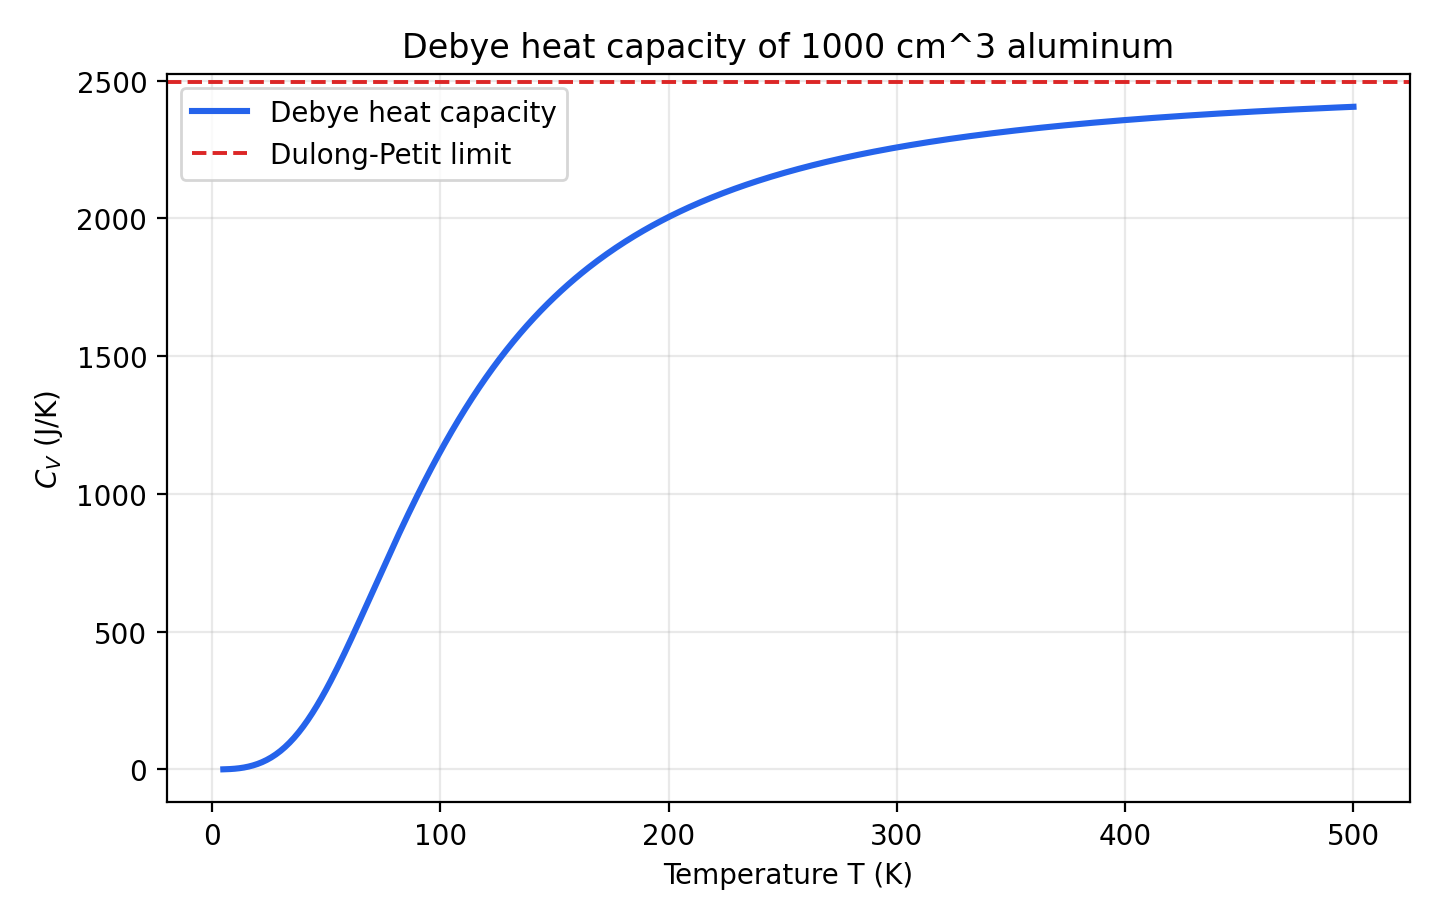
\includegraphics[width=0.82\linewidth,height=0.78\textheight,keepaspectratio,alt={Problem 1 heat capacity}]{../../../result/problem1_heat_capacity.png}
\caption{Problem 1 heat capacity}
\end{figure}

\subsubsection{分析}\label{ux5206ux6790-1}

结果符合 Debye 模型的定性预期：低温区热容很小，并随温度快速增长；高温区逐渐趋近 Dulong-Petit 极限。对于本题给定样品，\(T=500\,\mathrm{K}\) 时的热容约为 \(2405.2365\,\mathrm{J/K}\)，已经达到高温极限的约 \(96.4\%\)，但仍未完全饱和。

\section*{II. 自适应积分}\label{ii.-ux81eaux9002ux5e94ux79efux5206}
\addcontentsline{toc}{section}{II. 自适应积分}

本组问题要求计算

\[
I=\int_0^1\sin^2(\sqrt{100x})\,dx.
\]

\subsection{Problem 2(a)：自适应梯形积分}\label{problem-2a}

\scriptlink{problem2.py}

\subsubsection{待求问题}\label{ux5f85ux6c42ux95eeux9898-2}

编写程序，使用自适应梯形法将积分计算到近似精度 \(\epsilon=10^{-10}\)。从一个积分切片开始，每次将切片数加倍为 \(2,4,8,\ldots\)，并从 \(N=2\) 开始输出切片数、积分估计和误差估计，直到达到目标精度。题面提示结果应在 \(I=0.45\) 附近。

\subsubsection{解决方式}\label{ux89e3ux51b3ux65b9ux5f0f-2}

梯形法在第 \(i\) 级的切片数为 \(N_i=2^i\)，对应积分估计记为 \(T_i\)。相邻两级的误差估计采用

\[
\varepsilon_i^{(T)}\approx \frac{1}{3}|T_i-T_{i-1}|.
\]

自适应梯形法的计算流程如下：

\begin{verbatim}
Input : f(x) = sin^2(sqrt(100 x)), interval [0, 1], target eps
Output: final integral estimate and iteration history

T_prev <- trapezoid(f, 0, 1, 1)
for k = 1, 2, 3, ... do
    N <- 2^k
    T <- trapezoid(f, 0, 1, N)
    error <- |T - T_prev| / 3
    print N, T, error
    if error < eps then
        stop and return T
    end if
    T_prev <- T
end for
\end{verbatim}

\subsubsection{问题答案}\label{ux95eeux9898ux7b54ux6848-2}

自适应梯形法最终在 \(N=524288\) 时满足 \(\epsilon=10^{-10}\)。积分估计为

\[
I_T=0.455832532280153,
\]

误差估计为 \(2.893\times10^{-11}\)，与解析值的实际误差同为 \(2.893\times10^{-11}\)。

\subsubsection{分析}\label{ux5206ux6790-2}

Simpson 法只需要 \(2048\) 个切片，而梯形法需要 \(524288\) 个切片。二者相差 \(256\) 倍，说明 Simpson 法利用了更高阶的误差抵消，能够在同样目标精度下显著减少函数求值次数。粗网格阶段 Simpson 估计并非单调逼近，这是因为被积函数在 \([0,1]\) 上含有振荡结构；当网格足够细后，误差估计稳定下降并满足目标阈值。

\subsection{Problem 2(b)：自适应 Simpson 积分}\label{problem-2b}

\scriptlink{problem2.py}

\subsubsection{待求问题}\label{ux5f85ux6c42ux95eeux9898-3}

修改程序，使用自适应 Simpson 法计算同一积分，同样达到 \(\epsilon=10^{-10}\)。输出格式与 (a) 相同，并说明 Simpson 法是否以显著更少的切片数达到精度，以及这是否符合预期。

\subsubsection{解决方式}\label{ux89e3ux51b3ux65b9ux5f0f-3}

自适应 Simpson 法由相邻两级梯形估计组合得到

\[
S_i=\frac{4T_i-T_{i-1}}{3},
\]

并使用

\[
\varepsilon_i^{(S)}\approx \frac{1}{15}|S_i-S_{i-1}|
\]

作为误差估计。对应流程如下：

\begin{verbatim}
Input : f(x) = sin^2(sqrt(100 x)), interval [0, 1], target eps
Output: final Simpson estimate and iteration history

T_prev <- trapezoid(f, 0, 1, 1)
S_prev <- undefined
for k = 1, 2, 3, ... do
    N <- 2^k
    T <- trapezoid(f, 0, 1, N)
    S <- (4 T - T_prev) / 3
    if S_prev exists then
        error <- |S - S_prev| / 15
        print N, S, error
        if error < eps then
            stop and return S
        end if
    end if
    T_prev <- T
    S_prev <- S
end for
\end{verbatim}

为检查两种算法的输出，本题通过代换 \(u=\sqrt{100x}\) 得到解析参考值：

\[
I=\frac{1}{50}\int_0^{10}u\sin^2u\,du
=\frac12-\frac{\sin 20}{20}+\frac{1-\cos20}{400}
=0.455832532309085.
\]

\subsubsection{问题答案}\label{ux95eeux9898ux7b54ux6848-3}

自适应 Simpson 法最终在 \(N=2048\) 时满足 \(\epsilon=10^{-10}\)。积分估计为

\[
I_S=0.455832532224721,
\]

误差估计为 \(8.436\times10^{-11}\)，与解析值的实际误差也为 \(8.436\times10^{-11}\)。

两种方法的收敛过程如图 2 所示。

\begin{figure}
\centering
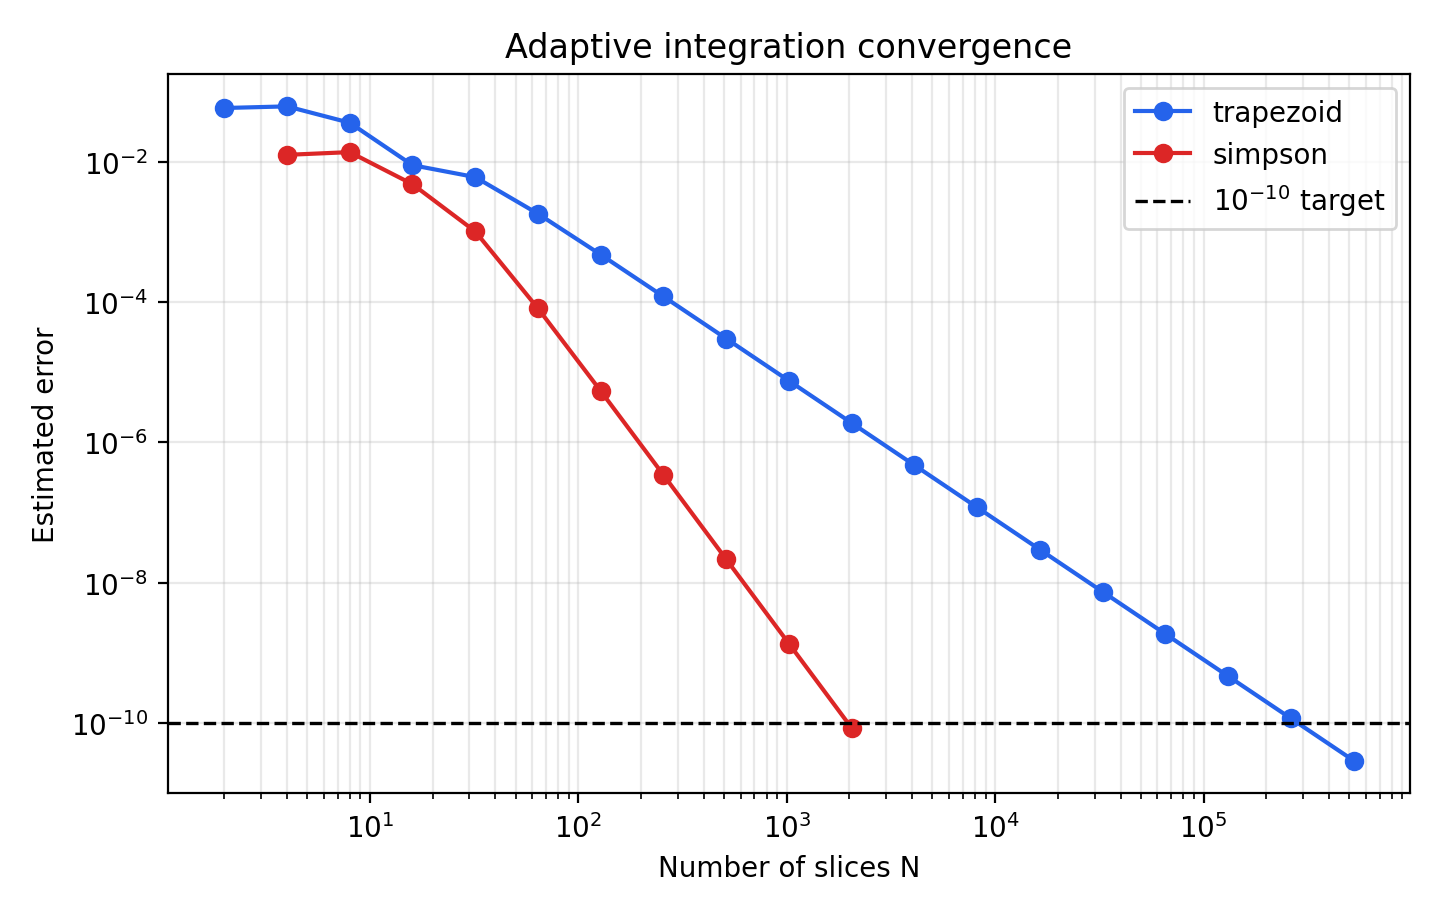
\includegraphics[width=0.8\linewidth,height=0.78\textheight,keepaspectratio,alt={Problem 2 adaptive convergence}]{../../../result/problem2_adaptive_convergence.png}
\caption{Problem 2 adaptive convergence}
\end{figure}

最终结果汇总如下。

\begin{table}[H]
  \centering
  \small
  \setlength{\tabcolsep}{5pt}
  \begin{tabular}{lrrrr}
    \toprule
    方法 & 达标 \(N\) & 积分估计 & 误差估计 & 实际误差 \\
    \midrule
    梯形 & 524288 & 0.455832532280153 & \(2.893\times10^{-11}\) & \(2.893\times10^{-11}\) \\
    Simpson & 2048 & 0.455832532224721 & \(8.436\times10^{-11}\) & \(8.436\times10^{-11}\) \\
    \bottomrule
  \end{tabular}
\end{table}

\subsubsection{分析}\label{ux5206ux6790-3}

Simpson 法只需要 \(2048\) 个切片，而梯形法需要 \(524288\) 个切片。二者相差 \(256\) 倍，说明 Simpson 法利用了更高阶的误差抵消，能够在同样目标精度下显著减少函数求值次数。粗网格阶段 Simpson 估计并非单调逼近，这是因为被积函数在 \([0,1]\) 上含有振荡结构；当网格足够细后，误差估计稳定下降并满足目标阈值。

\section*{III. 三种积分方法的误差关系}\label{iii.-ux4e09ux79cdux79efux5206ux65b9ux6cd5ux7684ux8befux5deeux5173ux7cfb}
\addcontentsline{toc}{section}{III. 三种积分方法的误差关系}

本组问题要求编写代码计算

\[
I=\int_0^1\frac{dx}{1+x^2}=\frac{\pi}{4},
\]

并分别用以下方法达到 \(\epsilon=10^{-2},10^{-3},10^{-4},\ldots,10^{-12}\) 的近似精度。

\subsection{Problem 3(a)：梯形法误差检验}\label{problem-3a}

\scriptlink{problem3.py}

\subsubsection{待求问题}\label{ux5f85ux6c42ux95eeux9898-4}

使用梯形法。

\subsubsection{解决方式}\label{ux89e3ux51b3ux65b9ux5f0f-4}

复合梯形法使用均匀网格，步长为 \(h=1/N\)，公式为

\[
T_N=h\left[\frac{f(x_0)+f(x_N)}{2}+\sum_{j=1}^{N-1}f(x_j)\right].
\]

计算流程如下：

\begin{verbatim}
Input : tolerance list eps_list, exact value pi / 4
Output: first N that satisfies each tolerance

for each eps in eps_list do
    for N = 1, 2, 4, 8, ... do
        value <- composite_trapezoid(f, 0, 1, N)
        error <- |value - pi / 4|
        if error < eps then
            record eps, N, value, error
            break
        end if
    end for
end for
\end{verbatim}

\subsubsection{问题答案}\label{ux95eeux9898ux7b54ux6848-4}

梯形法达到 \(10^{-12}\) 精度时需要 \(N=262144\)，此时

\[
I_T=0.7853981633968420,
\qquad
|I_T-\pi/4|=6.063234\times10^{-13}.
\]

\subsection{Problem 3(b)：Simpson 法误差检验}\label{problem-3b}

\scriptlink{problem3.py}

\subsubsection{待求问题}\label{ux5f85ux6c42ux95eeux9898-5}

使用 Simpson 法。

\subsubsection{解决方式}\label{ux89e3ux51b3ux65b9ux5f0f-5}

复合 Simpson 法仍使用均匀网格，但 \(N\) 必须为偶数，公式为

\[
S_N=\frac{h}{3}\left[f(x_0)+f(x_N)
+4\sum_{j=1,3,\ldots,N-1}f(x_j)
+2\sum_{j=2,4,\ldots,N-2}f(x_j)\right].
\]

计算流程如下：

\begin{verbatim}
Input : tolerance list eps_list, exact value pi / 4
Output: first even N that satisfies each tolerance

for each eps in eps_list do
    for N = 2, 4, 8, 16, ... do
        value <- composite_simpson(f, 0, 1, N)
        error <- |value - pi / 4|
        if error < eps then
            record eps, N, value, error
            break
        end if
    end for
end for
\end{verbatim}

\subsubsection{问题答案}\label{ux95eeux9898ux7b54ux6848-5}

Simpson 法达到 \(10^{-12}\) 精度时只需 \(N=64\)，此时

\[
I_S=0.7853981633973040,
\qquad
|I_S-\pi/4|=1.443596\times10^{-13}.
\]

\subsection{Problem 3(c)：Romberg 积分与误差平台}\label{problem-3c}

\scriptlink{problem3.py}

\subsubsection{待求问题}\label{ux5f85ux6c42ux95eeux9898-6}

使用 Romberg 积分。

题目还要求对每种方法测试误差关系，提示可以将误差拟合为步长 \(h\) 的幂律；如果误差关系不满足理论预期，需要给出解释。

\subsubsection{解决方式}\label{ux89e3ux51b3ux65b9ux5f0f-6}

Romberg 积分从梯形法序列出发，通过 Richardson 外推构造表

\[
R_{k,0}=T_{2^k},
\qquad
R_{k,j}=R_{k,j-1}+
\frac{R_{k,j-1}-R_{k-1,j-1}}{4^j-1}.
\]

计算流程如下：

\begin{verbatim}
Input : maximum level K, exact value pi / 4
Output: Romberg table and first N for each tolerance

for k = 0, 1, ..., K do
    R[k, 0] <- composite_trapezoid(f, 0, 1, 2^k)
    for j = 1, 2, ..., k do
        R[k, j] <- R[k, j-1] + (R[k, j-1] - R[k-1, j-1]) / (4^j - 1)
    end for
end for

for each eps in eps_list do
    find the first diagonal value R[k, k] with |R[k, k] - pi / 4| < eps
end for
\end{verbatim}

三种方法的误差阶检验统一采用

\[
|I_h-I|\approx Ch^p,
\]

即对 \(\log |I_h-I|\) 和 \(\log h\) 做线性拟合，斜率即为观测阶 \(p\)。为了观察步长继续减小时的数值现象，本报告把误差关系图的横轴从原先的 \(h\ge 2^{-16}\) 继续延长到

\[
h=2^{-28},\qquad N=268435456.
\]

同时，误差不再只与双精度 \texttt{math.pi/4} 比较，而是与高精度 \(\pi/4\) 常数比较。这样可以避免当积分结果恰好舍入到双精度 \(\pi/4\) 时误差被显示为 \(0\)，从而更清楚地观察机器精度平台。

\subsubsection{问题答案}\label{ux95eeux9898ux7b54ux6848-6}

Romberg 对角线达到 \(10^{-12}\) 精度时也在 \(N=64\) 达标，结果为

\[
I_R=0.7853981633974304,
\qquad
|I_R-\pi/4|=1.790521\times10^{-14}.
\]

达到各精度阈值所需的最小切片数如下。表中误差均为相对精确值 \(\pi/4\) 的绝对误差。

{\def\LTcaptype{none} % do not increment counter
\begin{longtable}[]{@{}
  >{\raggedright\arraybackslash}p{(\linewidth - 6\tabcolsep) * \real{0.2500}}
  >{\raggedright\arraybackslash}p{(\linewidth - 6\tabcolsep) * \real{0.2500}}
  >{\raggedright\arraybackslash}p{(\linewidth - 6\tabcolsep) * \real{0.2500}}
  >{\raggedright\arraybackslash}p{(\linewidth - 6\tabcolsep) * \real{0.2500}}@{}}
\toprule\noalign{}
\begin{minipage}[b]{\linewidth}\raggedright
\(\epsilon\)
\end{minipage} & \begin{minipage}[b]{\linewidth}\raggedright
梯形法 \(N\) / 误差
\end{minipage} & \begin{minipage}[b]{\linewidth}\raggedright
Simpson 法 \(N\) / 误差
\end{minipage} & \begin{minipage}[b]{\linewidth}\raggedright
Romberg \(N\) / 误差
\end{minipage} \\
\midrule\noalign{}
\endhead
\bottomrule\noalign{}
\endlastfoot
\(10^{-2}\) & 4 / \(2.604046\times10^{-3}\) & 2 / \(2.064830\times10^{-3}\) & 2 / \(2.064830\times10^{-3}\) \\
\(10^{-3}\) & 8 / \(6.510398\times10^{-4}\) & 4 / \(6.006535\times10^{-6}\) & 4 / \(1.312484\times10^{-4}\) \\
\(10^{-4}\) & 32 / \(4.069010\times10^{-5}\) & 4 / \(6.006535\times10^{-6}\) & 8 / \(1.717457\times10^{-6}\) \\
\(10^{-5}\) & 128 / \(2.543132\times10^{-6}\) & 4 / \(6.006535\times10^{-6}\) & 8 / \(1.717457\times10^{-6}\) \\
\(10^{-6}\) & 256 / \(6.357829\times10^{-7}\) & 8 / \(3.778277\times10^{-8}\) & 16 / \(2.921981\times10^{-9}\) \\
\(10^{-7}\) & 1024 / \(3.973643\times10^{-8}\) & 8 / \(3.778277\times10^{-8}\) & 16 / \(2.921981\times10^{-9}\) \\
\(10^{-8}\) & 2048 / \(9.934107\times10^{-9}\) & 16 / \(5.912429\times10^{-10}\) & 16 / \(2.921981\times10^{-9}\) \\
\(10^{-9}\) & 8192 / \(6.208817\times10^{-10}\) & 16 / \(5.912429\times10^{-10}\) & 32 / \(1.211261\times10^{-11}\) \\
\(10^{-10}\) & 32768 / \(3.880510\times10^{-11}\) & 32 / \(9.239196\times10^{-12}\) & 32 / \(1.211261\times10^{-11}\) \\
\(10^{-11}\) & 65536 / \(9.701270\times10^{-12}\) & 32 / \(9.239196\times10^{-12}\) & 64 / \(1.790521\times10^{-14}\) \\
\(10^{-12}\) & 262144 / \(6.063234\times10^{-13}\) & 64 / \(1.443596\times10^{-13}\) & 64 / \(1.790521\times10^{-14}\) \\
\end{longtable}
}

延长横轴后的误差与步长双对数关系如图 3 所示。横轴最右端对应 \(h=2^{-28}\)，灰色虚线为双精度机器精度量级。

\begin{figure}
\centering
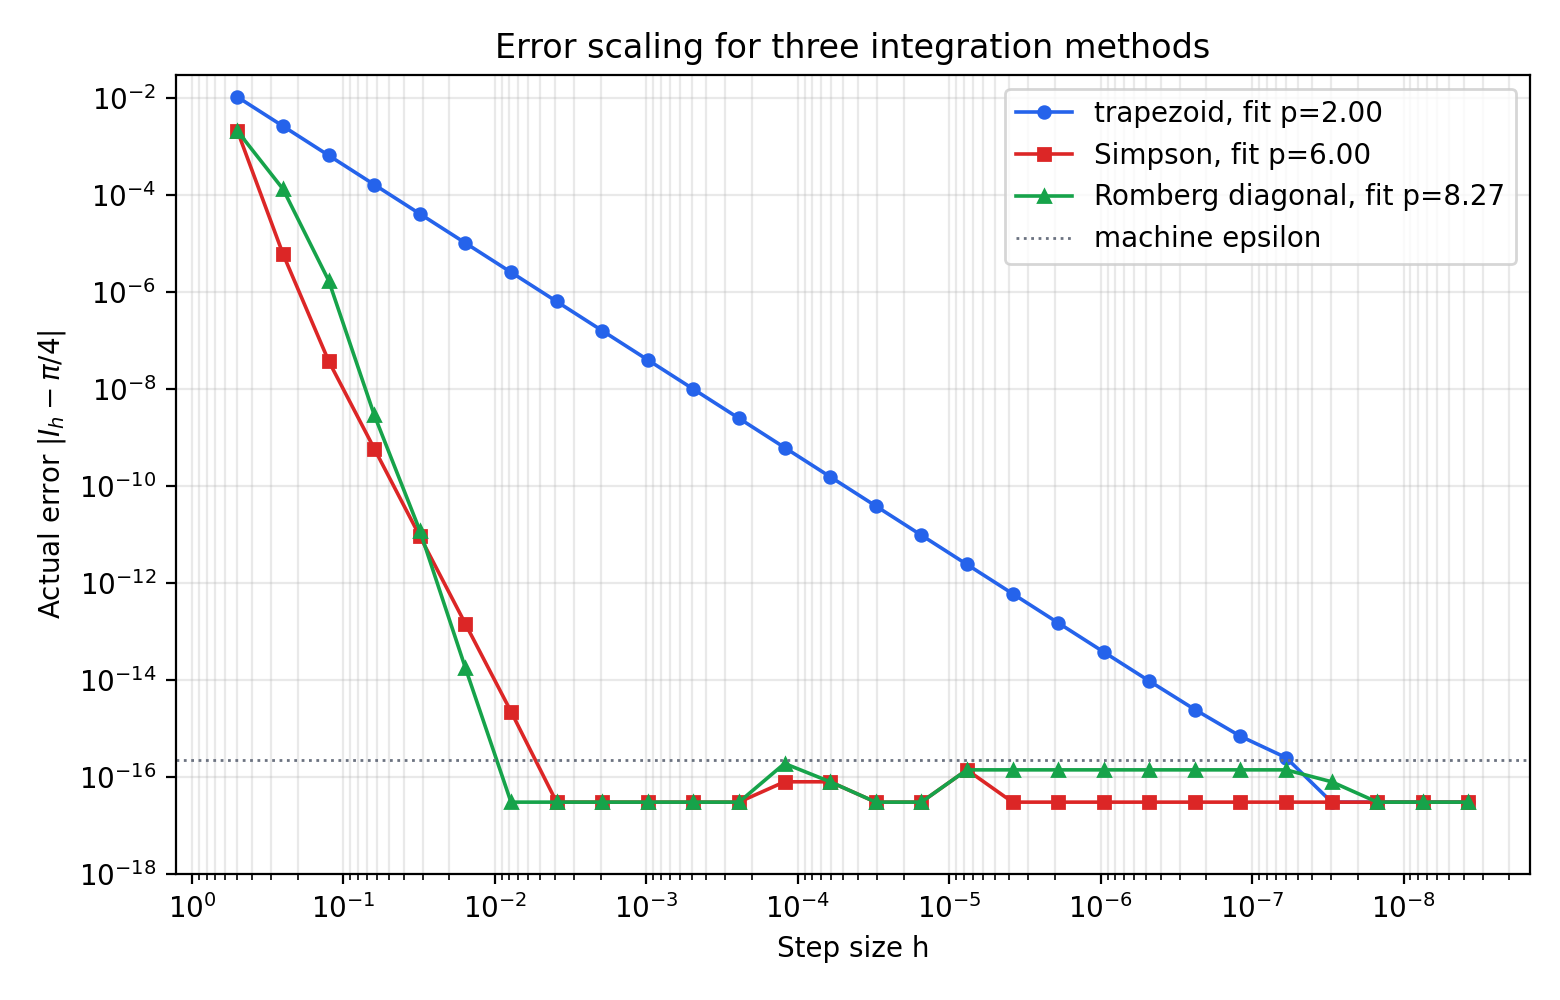
\includegraphics[width=0.82\linewidth,height=0.78\textheight,keepaspectratio,alt={Problem 3 error scaling}]{../../../result/problem3_error_scaling.png}
\caption{Problem 3 error scaling}
\end{figure}

为了更清楚地观察机器精度附近的行为，图 4 只保留小步长区间。可以看到 Simpson 法和 Romberg 法早已进入舍入平台，梯形法继续二阶下降一段后也到达同一平台。

\begin{figure}
\centering
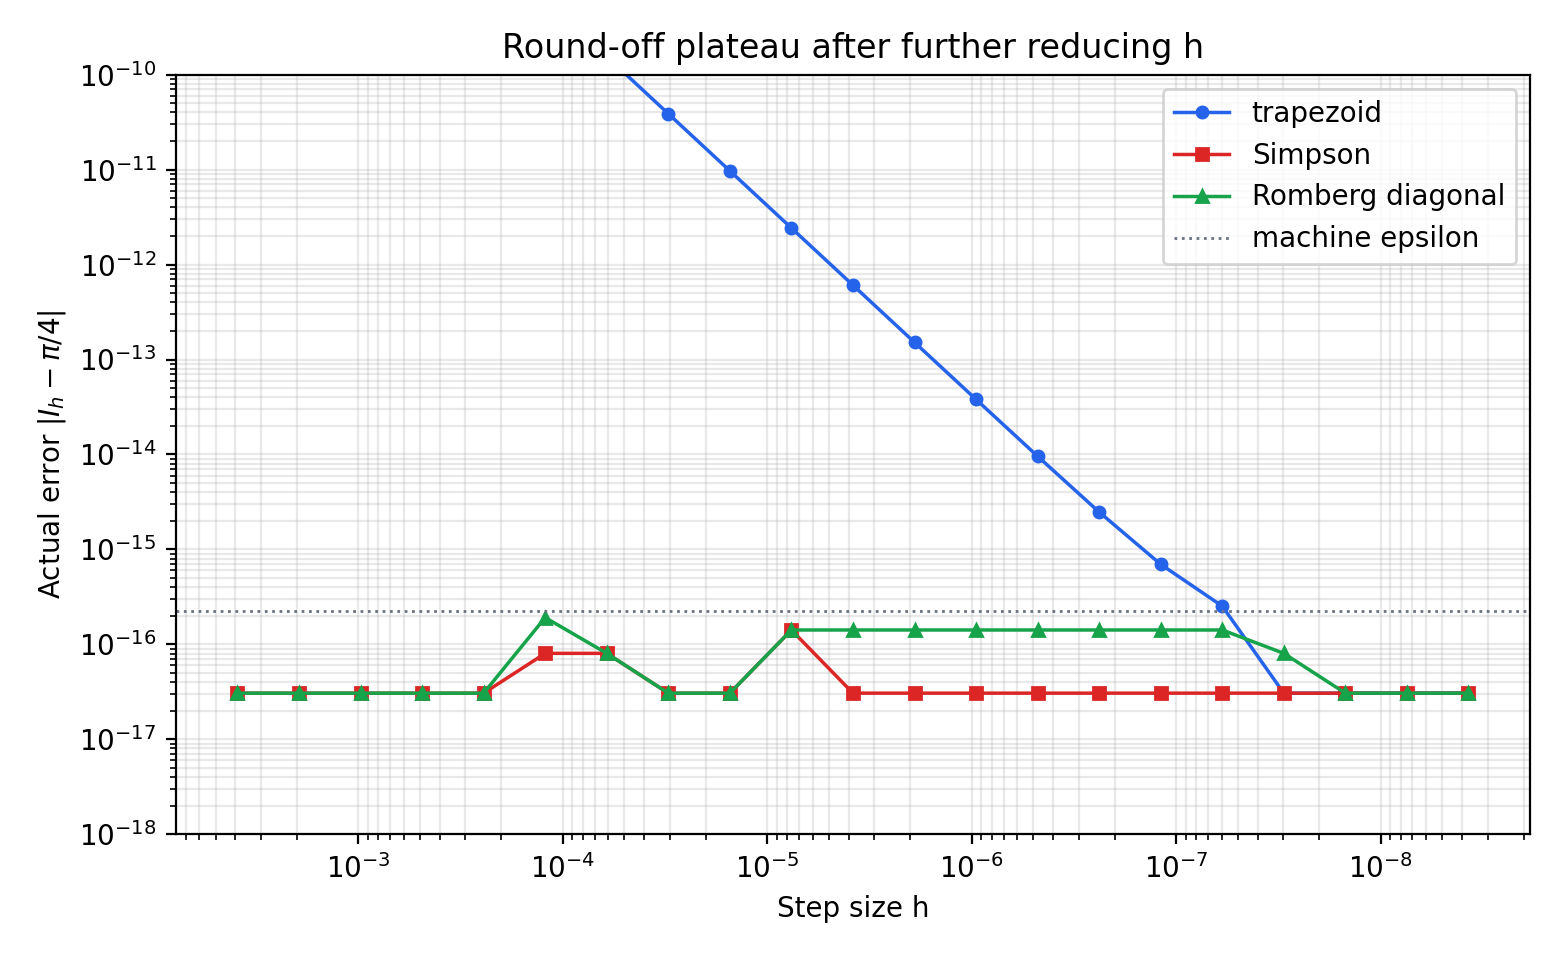
\includegraphics[width=0.82\linewidth,height=0.78\textheight,keepaspectratio,alt={Problem 3 round-off zoom}]{../../../result/problem3_roundoff_zoom.png}
\caption{Problem 3 round-off zoom}
\end{figure}

拟合得到的观测阶为：

{\def\LTcaptype{none} % do not increment counter
\begin{longtable}[]{@{}
  >{\raggedright\arraybackslash}p{(\linewidth - 4\tabcolsep) * \real{0.3333}}
  >{\raggedleft\arraybackslash}p{(\linewidth - 4\tabcolsep) * \real{0.3333}}
  >{\raggedright\arraybackslash}p{(\linewidth - 4\tabcolsep) * \real{0.3333}}@{}}
\toprule\noalign{}
\begin{minipage}[b]{\linewidth}\raggedright
方法
\end{minipage} & \begin{minipage}[b]{\linewidth}\raggedleft
观测阶 \(p\)
\end{minipage} & \begin{minipage}[b]{\linewidth}\raggedright
解释
\end{minipage} \\
\midrule\noalign{}
\endhead
\bottomrule\noalign{}
\endlastfoot
梯形法 & 1.9999 & 与复合梯形法 \(O(h^2)\) 的标准误差关系一致。 \\
Simpson 法 & 5.9993 & 高于一般情形的 \(O(h^4)\)，原因是本题函数使 Simpson 公式的主误差项抵消。 \\
Romberg 对角线 & 8.2674 & Romberg 每一列都在消去更低阶误差项，因此不应期待单一固定幂律。 \\
\end{longtable}
}

延长横轴后可观察到的末端现象如下。

{\def\LTcaptype{none} % do not increment counter
\begin{longtable}[]{@{}
  >{\raggedright\arraybackslash}p{(\linewidth - 8\tabcolsep) * \real{0.2000}}
  >{\raggedleft\arraybackslash}p{(\linewidth - 8\tabcolsep) * \real{0.2000}}
  >{\raggedleft\arraybackslash}p{(\linewidth - 8\tabcolsep) * \real{0.2000}}
  >{\raggedleft\arraybackslash}p{(\linewidth - 8\tabcolsep) * \real{0.2000}}
  >{\raggedright\arraybackslash}p{(\linewidth - 8\tabcolsep) * \real{0.2000}}@{}}
\toprule\noalign{}
\begin{minipage}[b]{\linewidth}\raggedright
方法
\end{minipage} & \begin{minipage}[b]{\linewidth}\raggedleft
最小误差对应 \(N\)
\end{minipage} & \begin{minipage}[b]{\linewidth}\raggedleft
最小误差
\end{minipage} & \begin{minipage}[b]{\linewidth}\raggedleft
\(N=268435456\) 时误差
\end{minipage} & \begin{minipage}[b]{\linewidth}\raggedright
现象
\end{minipage} \\
\midrule\noalign{}
\endhead
\bottomrule\noalign{}
\endlastfoot
梯形法 & 33554432 & \(3.061617\times10^{-17}\) & \(3.061617\times10^{-17}\) & 截断误差继续二阶下降，最终也落到双精度舍入平台。 \\
Simpson 法 & 256 & \(3.061617\times10^{-17}\) & \(3.061617\times10^{-17}\) & 很早达到双精度可分辨极限，继续减小 \(h\) 不再带来收益。 \\
Romberg 对角线 & 128 & \(3.061617\times10^{-17}\) & \(3.061617\times10^{-17}\) & 外推快速达到机器精度，末端只剩舍入平台上的小幅浮动。 \\
\end{longtable}
}

\subsection{Problem 3：综合分析}\label{problem-3-analysis}

梯形法的结果最直接地验证了二阶收敛。Simpson 法通常具有 \(O(h^4)\) 精度，但本题的

\[
f(x)=\frac{1}{1+x^2}
\]

满足

\[
f'''(x)=\frac{24x(1-x^2)}{(1+x^2)^4},\qquad f'''(0)=f'''(1)=0.
\]

复合 Simpson 公式的 \(h^4\) 主误差项与端点三阶导数差有关，因此该项在本题中消失，实际进入 \(O(h^6)\) 主导区。这解释了观测阶约为 \(6\)，并不是程序错误。

延长横轴后，误差曲线不能继续按幂律无限下降。数值积分的总误差可概括为

\[
E(h)\approx C_{\mathrm{trunc}}h^p+C_{\mathrm{round}}\varepsilon_{\mathrm{mach}}h^{-q},
\]

其中第一项是离散截断误差，随 \(h\) 减小而下降；第二项来自函数值求和、相近数相减和 Richardson 外推中的舍入误差，通常会在 \(N\) 很大时累积或被放大。梯形法的截断误差为二阶，因此下降较慢；继续延长到 \(h=2^{-28}\) 后，梯形法也进入 \(10^{-17}\) 到 \(10^{-16}\) 的双精度平台。Simpson 法在本题中呈六阶下降，很快达到双精度能够表示的极限；此后继续增加切片只是在重复得到同一个或相邻的双精度数。Romberg 方法虽然在粗网格到中等网格上收敛最快，但外推公式不断使用相邻近似值的差来消去低阶项，当这些差已经接近舍入误差时，外推结果不再代表真实截断误差的下降，而是在同一个舍入平台附近波动。

图中的平台略低于机器精度虚线并不矛盾。机器精度 \(\varepsilon_{\mathrm{mach}}\approx2.22\times10^{-16}\) 描述的是双精度相对间距的量级，而一个具体数值舍入到最近浮点数时，绝对误差可以小于该量级。本题中双精度表示的 \(\pi/4\) 与高精度真值之间的差约为 \(3.06\times10^{-17}\)，因此 Simpson 法和 Romberg 法的最低平台正好落在这一水平附近。

\section*{IV. 可换元积分}\label{iv.-ux53efux6362ux5143ux79efux5206}
\addcontentsline{toc}{section}{IV. 可换元积分}

本组问题要求使用课堂讨论的方法编写代码，计算下列积分。

\subsection{Problem 4(a)：半圆面积积分}\label{problem-4a}

\scriptlink{problem4.py}

\subsubsection{待求问题}\label{ux5f85ux6c42ux95eeux9898-7}

\[
I=\int_{-1}^{1}\sqrt{1-x^2}\,dx.
\]

\subsubsection{解决方式}\label{ux89e3ux51b3ux65b9ux5f0f-7}

直接对 \(\sqrt{1-x^2}\) 积分会遇到端点导数奇性。令

\[
x=\sin\theta,\qquad \theta\in[-\pi/2,\pi/2],
\]

则

\[
\sqrt{1-x^2}\,dx=\cos^2\theta\,d\theta.
\]

于是原积分化为

\[
I=\int_{-\pi/2}^{\pi/2}\cos^2\theta\,d\theta.
\]

\subsubsection{问题答案}\label{ux95eeux9898ux7b54ux6848-7}

经 \(x=\sin\theta\) 代换后，数值结果为

\[
I=1.5707963267948966=\frac{\pi}{2},
\]

显示误差为 \(0.0\)。

\subsubsection{分析}\label{ux5206ux6790-7}

三项结果均在双精度显示范围内与理论值一致。关键并不只是增大切片数，而是先通过变量代换改善被积函数结构。特别是 (c) 中的无穷上限和 \(\sqrt{x}\) 奇性同时消失，变成常数积分后无需依赖很大的截断区间。

\subsection{Problem 4(b)：正弦平方积分}\label{problem-4b}

\scriptlink{problem4.py}

\subsubsection{待求问题}\label{ux5f85ux6c42ux95eeux9898-8}

\[
I=\int_0^\pi\sin^2\theta\,d\theta.
\]

\subsubsection{解决方式}\label{ux89e3ux51b3ux65b9ux5f0f-8}

该积分已经位于有限光滑区间，直接使用复合 Simpson 法计算

\[
I=\int_0^\pi\sin^2\theta\,d\theta.
\]

\subsubsection{问题答案}\label{ux95eeux9898ux7b54ux6848-8}

直接积分得到

\[
I=1.5707963267948966=\frac{\pi}{2},
\]

显示误差为 \(0.0\)。

\subsubsection{分析}\label{ux5206ux6790-8}

三项结果均在双精度显示范围内与理论值一致。关键并不只是增大切片数，而是先通过变量代换改善被积函数结构。特别是 (c) 中的无穷上限和 \(\sqrt{x}\) 奇性同时消失，变成常数积分后无需依赖很大的截断区间。

\subsection{Problem 4(c)：无穷区间奇性积分}\label{problem-4c}

\scriptlink{problem4.py}

\subsubsection{待求问题}\label{ux5f85ux6c42ux95eeux9898-9}

\[
I=\int_0^\infty\frac{1}{(1+x)\sqrt{x}}\,dx.
\]

\subsubsection{解决方式}\label{ux89e3ux51b3ux65b9ux5f0f-9}

该积分同时有无穷上限和 \(x=0\) 处的奇性。令

\[
x=\tan^2\theta,\qquad \theta\in[0,\pi/2],
\]

则

\[
dx=2\tan\theta\sec^2\theta\,d\theta,
\qquad
(1+x)\sqrt{x}=\sec^2\theta\tan\theta,
\]

因此原积分化为

\[
I=\int_0^{\pi/2}2\,d\theta.
\]

三项积分在程序中的统一流程如下：

\begin{verbatim}
Input : transformed integrands and exact reference values
Output: numerical estimates and absolute errors

cases <- [
    (a, cos(theta)^2, -pi/2, pi/2, pi/2),
    (b, sin(theta)^2, 0, pi, pi/2),
    (c, 2, 0, pi/2, pi)
]

for each case do
    value <- composite_simpson(transformed_integrand, left, right, 1024)
    error <- |value - exact|
    record case, transformation, value, exact, error
end for
\end{verbatim}

\subsubsection{问题答案}\label{ux95eeux9898ux7b54ux6848-9}

经 \(x=\tan^2\theta\) 代换后，数值结果为

\[
I=3.1415926535897931=\pi,
\]

显示误差为 \(0.0\)。

结果汇总如下。

{\def\LTcaptype{none} % do not increment counter
\begin{longtable}[]{@{}llrrr@{}}
\toprule\noalign{}
小问 & 变量代换 & 数值结果 & 理论值 & 绝对误差 \\
\midrule\noalign{}
\endhead
\bottomrule\noalign{}
\endlastfoot
(a) & \(x=\sin\theta\) & 1.5707963267948966 & \(\pi/2\) & \(0.0\) \\
(b) & 直接积分 & 1.5707963267948966 & \(\pi/2\) & \(0.0\) \\
(c) & \(x=\tan^2\theta\) & 3.1415926535897931 & \(\pi\) & \(0.0\) \\
\end{longtable}
}

\subsubsection{分析}\label{ux5206ux6790-9}

三项结果均在双精度显示范围内与理论值一致。关键并不只是增大切片数，而是先通过变量代换改善被积函数结构。特别是 (c) 中的无穷上限和 \(\sqrt{x}\) 奇性同时消失，变成常数积分后无需依赖很大的截断区间。

\section*{V. n 维单位超球体积}\label{v.-n-ux7ef4ux5355ux4f4dux8d85ux7403ux4f53ux79ef}
\addcontentsline{toc}{section}{V. n 维单位超球体积}

本组问题要求估计单位半径超球体积随维数变化的关系。二维情形可写作

\[
I=\int_{-1}^{1}\int_{-1}^{1} f(x,y)\,dx\,dy,
\]

其中

\[
f(x,y)=
\begin{cases}
1, & x^2+y^2\le 1,\\
0, & \text{otherwise}.
\end{cases}
\]

题面还给出解析公式

\[
V_n=\frac{\pi^{n/2}R^n}{\Gamma(n/2+1)}=C_nR^n,
\]

其中 \(\Gamma\) 为 Gamma 函数。本题中该公式只用于运行后的相对误差核对，不作为体积估计的生成方法。

\subsection{Problem 5(a)：直接直角坐标积分与 30 维结果}\label{problem-5a}

\scriptlink{problem5_direct_cartesian/}

\subsubsection{待求问题}\label{ux5f85ux6c42ux95eeux9898-10}

计算单位超球体积，并将可计算维数至少推进到 \(n=28\)。同时说明在不依赖体积递推、Monte Carlo 或同类随机近似的条件下，怎样继续推进到 \(30\) 维附近。

\subsubsection{解决方式}\label{ux89e3ux51b3ux65b9ux5f0f-10}

半径取 \(R=1\)。本题主数值结果不使用 Monte Carlo、体积递推关系、Gamma 闭式公式、球坐标变量代换、动态规划计数、bitset 压缩算子或边界剪枝，而是从直角坐标积分定义出发：

\[
V_n=\int_{[-1,1]^n}\mathbf{1}_{x_1^2+\cdots+x_n^2\le 1}\,dx_1\cdots dx_n .
\]

唯一使用的数学化简是坐标符号对称性：

\[
V_n=2^n\int_{[0,1]^n}\mathbf{1}_{x_1^2+\cdots+x_n^2\le 1}\,dx_1\cdots dx_n .
\]

这一步只把 \(2^n\) 个对称卦限合并，不改变被积函数，也不把问题降成一维径向积分。第一卦限上采用复合中点张量公式。若第 \(i\) 个坐标轴划分为 \(q_i\) 个中点小区间，则

\[
x_{i,k_i}=\frac{2k_i+1}{2q_i},\qquad k_i=0,\ldots,q_i-1.
\]

于是混合分辨率直角中点公式为

\[
\widehat V_n
=2^n\left(\prod_{i=1}^n\frac{1}{q_i}\right)
\sum_{k_1=0}^{q_1-1}\cdots\sum_{k_n=0}^{q_n-1}
\mathbf{1}_{\sum_i x_{i,k_i}^2\le 1}.
\]

记
\[
P(\mathbf q)=\prod_{i=1}^n q_i,\qquad
C(\mathbf q)=
\#\left\{(k_1,\ldots,k_n):\sum_i x_{i,k_i}^2\le 1\right\}.
\]
则中点张量公式可以写成
\[
\widehat V_n=2^n\frac{C(\mathbf q)}{P(\mathbf q)}.
\]
因此程序的核心任务不是求 Gamma 函数或递推体积，而是在给定直角中点网格上直接得到球内点数
\(C(\mathbf q)\)。这个表达式也说明了计算困难：若所有坐标都取同一分辨率
\(q\)，则第一卦限点数为 \(q^n\)，维数每增加一维都会把工作量再乘以
\(q\)。

实际推进时，本题把工作拆成三个层次。第一层是数学边界：只允许使用直角中点张量积分、符号对称性和等价整数判定，避免把最终答案变成递推公式、Gamma 闭式值、随机抽样或半径层动态规划。第二层是候选网格筛选：在真正启动高维 direct run 之前，先用系数计数器快速判断哪些混合 \(q\)-pattern 有希望满足误差阈值，并把不可承受的组合排除。第三层是 strict kernel 验证：选中的少数候选仍必须由逐点 prefix--tail 比较得到 inside count，且工程优化需要通过消融测试证明没有改变积分公式。这三个层次分别对应“可算什么”“值得算什么”和“最终怎样算出来”。

需要注意的是，被积函数是球指标函数，在边界
\(\sum_i x_i^2=1\) 上有跃变。复合中点法对光滑函数常见的高阶余项估计不能直接套用到这里；主要误差来自被球面切开的直角小盒。高维下边界附近的小盒数量随维数和网格相位变化很敏感，因此误差可能随 \(q\)-pattern 非单调变化。本文采用中点公式的理由是它权重全为正、每个张量点含义清楚、并且可被严格整数化为点内外判定；误差控制则通过候选网格筛选和实际 direct run 后的相对误差核对完成。

为了在高维下控制计算量，本题没有强制每个坐标轴使用同一 \(q\)，而是允许 \(q_i\in\{2,3,4,5,6\}\)。例如

\[
2^1 3^{16}4^7 5^2 6^2
\]

表示第一卦限中有 \(1\) 个坐标轴取 \(q=2\)、\(16\) 个坐标轴取 \(q=3\)、\(7\) 个坐标轴取 \(q=4\)、\(2\) 个坐标轴取 \(q=5\)、\(2\) 个坐标轴取 \(q=6\)。这里的 \(q\) 是该坐标轴上的中点小区间数，不是插值阶数，也不是改变积分变量后的径向分层。混合分辨率的作用是把
\(P(\mathbf q)\) 压低，同时让部分坐标轴保留较细中点以减小边界相位误差。

在程序实现中，为避免浮点比较误差，点内外判定写成等价整数形式。因为 \(2,3,4,5,6\) 的最小公倍数为 \(60\)，对每个坐标有

\[
x_{i,k_i}=\frac{(2k_i+1)(60/q_i)}{120},
\]

所以球内条件等价为

\[
\sum_i\left((2k_i+1)\frac{60}{q_i}\right)^2\le 120^2.
\]

这一步只是把有限精度浮点比较换成完全等价的整数比较，不改变中点坐标，也不改变积分公式。由于半径阈值只有 \(120^2\)，每个坐标对半径平方的贡献可以预先存成小整数表，后续枚举时只做整数加减。

CPU 核心程序进一步采用 prefix--tail 执行布局。把坐标集合分为
\(A\) 和 \(B\)，对应 prefix 和 tail，并记
\[
P_A=\prod_{i\in A}q_i,\qquad P_B=\prod_{i\in B}q_i,\qquad
P_A P_B=P(\mathbf q).
\]
对一个 prefix 点 \(\alpha\) 和 tail 点 \(\beta\)，整数半径平方可写成
\[
S(\alpha,\beta)=S_A(\alpha)+S_B(\beta).
\]
于是球内点数仍是完整的二重枚举
\[
C(\mathbf q)=
\sum_{\alpha\in G_A}\sum_{\beta\in G_B}
\mathbf{1}_{S_B(\beta)\le 120^2-S_A(\alpha)}.
\]
程序先枚举并存储每个 tail 点的 \(S_B(\beta)\)，再枚举每个 prefix 点并计算剩余阈值
\(120^2-S_A(\alpha)\)。随后对每个 prefix 阈值逐项扫描整张 tail 主表。为降低内存带宽，tail 的不同半径平方值先被建立成无损 rank 字典，tail 主表保存每个 tail 点对应的 rank8 字节，AVX2 一次比较 \(32\) 个 tail rank。计数主循环不对 tail 点排序、不做二分查找、不合并半径层，也不跳过 prefix 或 tail 区域；每个 prefix--tail 对仍通过一次 rank 比较参与计数。

更具体地说，tail 表不是半径层计数表，而是一张按 tail 张量点逐项排列的数组。若
\[
G_B=\{\beta_0,\beta_1,\ldots,\beta_{P_B-1}\},
\]
则未压缩时保存
\[
T_j=S_B(\beta_j),\qquad j=0,\ldots,P_B-1.
\]
因为任意 prefix 的剩余阈值都不超过 \(120^2\)，所有
\(T_j>120^2\) 的条目在比较中必然失败，可以无损地饱和为同一个哨兵值
\(s_\infty>120^2\)。设
\[
U_B=\operatorname{uniqueSort}\{\,\min(T_j,s_\infty):0\le j<P_B\,\},
\]
表示先排序再去重得到的有序值表。rank8 主表实际保存的是
\[
R_j=\operatorname{rank}\bigl(\min(T_j,s_\infty)\bigr)\in\{0,\ldots,|U_B|-1\},
\]
同时预先保存每个 prefix 阈值 \(\tau\) 对应的
\[
B(\tau)=\#\{u\in U_B:u\le \tau\}.
\]
于是
\[
S_B(\beta_j)\le \tau\quad\Longleftrightarrow\quad R_j<B(\tau).
\]
这说明 rank8 只是把逐项整数比较改写成逐项字节 rank 比较，并没有把 tail 点合并成计数层。

最终 \(n=27,\ldots,30\) 使用的 tail 表配置如下。轴顺序为升序，即先放 \(q=2\)，再放
\(q=3,4,5,6\)，tail 取最后若干轴，因此 tail 侧主要包含较高分辨率坐标。

\begin{table}[H]
  \centering
  \normalsize
  \renewcommand{\arraystretch}{1.15}
  \setlength{\tabcolsep}{5pt}
  \begin{tabular}{r c l r r r}
    \toprule
    \(n\) & tail 维数 & tail 轴模式 & \(P_B\) & rank8 主表 & rank 值数 \\
    \midrule
    27 & 8  & \(4^5 6^3\)       & \(221184\)  & \(0.211\,\mathrm{MiB}\) & 54 \\
    28 & 8  & \(4^4 5^2 6^2\)   & \(230400\)  & \(0.220\,\mathrm{MiB}\) & 213 \\
    29 & 8  & \(4^6 6^2\)       & \(147456\)  & \(0.141\,\mathrm{MiB}\) & 45 \\
    30 & 10 & \(4^1 5^9\)       & \(7812500\) & \(7.451\,\mathrm{MiB}\) & 32 \\
    \bottomrule
  \end{tabular}
\end{table}

上表的 rank 值数已经包含 \(T_j>120^2\) 的饱和哨兵值。以 \(n=30\) 为例，tail 表有
\(4\cdot5^9=7812500\) 个字节级条目，构造时间为
\(0.071\,\mathrm{s}\)；而随后的 prefix--tail 逐点比较耗时
\(6681.206\,\mathrm{s}\)。因此 tail 表构造不是主要耗时，它的作用是把内层循环变成连续内存读取和 SIMD 字节比较。

计算流程如下：

\begin{verbatim}
Input : dimension n and mixed q-pattern
Output: direct midpoint tensor estimate

build all q_i axes in the first orthant
build integer squared-radius table for the tail axes
encode tail sums by lossless rank8 values

inside <- 0
for every prefix midpoint do
    remaining <- 120^2 - prefix_squared_radius
    for every tail midpoint do
        if tail_squared_radius <= remaining then
            inside <- inside + 1
        end if
    end for
end for

return 2^n * inside / product(q_i)
\end{verbatim}

上述 prefix--tail 写法本质上只是改变枚举顺序和中间量保存方式。原始张量点仍为
\((k_1,\ldots,k_n)\)，每一个 prefix 点都要同每一个 tail 点组成完整的
\(n\) 维直角中点并做一次半径比较。因此它不属于递推降维、稀疏网格或边界剪枝。
其时间复杂度仍为
\[
T=\Theta(P_A P_B)=\Theta(P(\mathbf q)),
\]
辅助内存主要为 \(O(P_B)\) 的 tail 表。tail 维数的选择只是在缓存容量、内存带宽和线程调度之间做工程折中；它不会减少要比较的张量点总数。

工程优化是本题能维持 \(2\times10^{12}\) points/s 以上吞吐量的关键。优化思路不是减少应枚举的张量点，而是把每个点的判定代价压到很低：

\begin{itemize}
\item \textbf{整数化半径。} 每个坐标的
\(\left((2k_i+1)60/q_i\right)^2\) 预先存入小表。混合进位枚举时，坐标变化只需要用新旧 digit 的平方贡献差更新当前半径平方，不重新对 \(n\) 个坐标求和，也不做开方、除法或浮点比较。
\item \textbf{tail 表复用。} tail 部分的半径平方只构造一次，之后被所有 prefix 点共享。这样内层循环只需要读连续 tail 数组并与当前阈值比较，不需要重复生成 tail 坐标。以 \(n=30\) 的最终参数为例，tail 维数取 \(10\)，tail 点数为 \(4\cdot5^9=7812500\)，rank8 后 tail 主表约为 \(7.8\) MB，适合连续扫描和多线程共享读取。
\item \textbf{rank8 无损压缩。} 由于 tail 半径平方只需要同阈值比较，程序先把所有不同的 tail 半径平方排序并映射为单字节 rank，同时保存 threshold 到 rank bound 的查表关系。比较
\(\text{tail\_sum}\le \text{remaining}\)
等价变成
\(\text{tail\_rank}<\text{rank\_bound}\)。
这一步是无损编码，仍逐个 tail 点比较，但把主循环读带宽从 u16 降到 u8。
\item \textbf{prefix batching。} 若一次只处理一个 prefix 阈值，tail 表会被反复单独扫描。最终程序把 \(16\) 个 prefix 阈值组成一批，对同一段 tail 数据同时做 \(16\) 组比较。这样一段 tail 数据被读入后可以服务多个 prefix 点，显著提高每字节内存访问对应的有效点比较数。
\item \textbf{AVX2 向量比较和手写展开。} rank8 主循环每次载入 \(32\) 个 tail rank。实际实现对 \(4\) 个连续 AVX2 向量做展开，因此在 \texttt{batch\_prefixes}=16 时，一个展开块对应 \(4\times32\times16=2048\) 个 prefix--tail 点比较。之后通过 movemask 和 popcount 累加命中数。由于 AVX2 的字节比较是有符号比较，程序用异或 \(0x80\) 的偏移把无符号 rank 比较转成等价的有符号比较。
\item \textbf{OpenMP 静态分块。} prefix 空间按固定 chunk 分给线程，tail 表只读共享，每个线程只维护自己的 prefix index 和局部计数，最后做 reduction。最终 \(n=27,\ldots,30\) 的 direct run 使用 \(88\) 个线程；构造 tail 表的时间相对于计数时间可以忽略，主要耗时都集中在可并行的内层比较。
\item \textbf{layout 参数实测。} tail 维数、prefix chunk、坐标顺序和 batch 大小都会影响缓存命中、寄存器压力和调度开销。测试显示 \texttt{batch\_prefixes}=32 在本机反而降低速度，说明过度展开会带来寄存器溢出和指令压力；最终路线使用 \texttt{batch\_prefixes}=16、rank8 storage 和针对候选网格选出的 tail 维数。
\end{itemize}

为了支撑这些工程优化，本题补充了独立的 ablation 测试。测试使用较小的 proxy 网格，保证所有对照仍在第一卦限直角中点张量上逐点比较；每组对照只改变一个主要实现因素，并检查球内点数是否一致。完整记录保存在如下两个 CSV 文件中：
\begin{center}
\begin{tabular}{@{}l@{}}
q23456\_engineering\_ablation\_raw.csv\\
q23456\_engineering\_ablation\_summary.csv
\end{tabular}
\end{center}
其中 raw 文件包含 \(60\) 条重复测量记录，summary 文件归并为 \(10\) 组主要对照。消融表的目的不是把所有倍率机械相乘，而是说明每一类实现选择都被单独检查过：有的优化提供数量级收益，例如整数增量半径、AVX2 展开和多线程；也有的选择只带来小幅改善，甚至出现负收益，例如 \texttt{batch\_prefixes}=32。这种负收益检查很重要，因为它说明最终参数不是“展开越多越好”的形式化调参，而是受寄存器压力、缓存行为和内存带宽共同限制。

\begin{table}[H]
  \centering
  \small
  \setlength{\tabcolsep}{2.5pt}
  \begin{tabular}{p{0.20\textwidth}p{0.26\textwidth}p{0.26\textwidth}p{0.14\textwidth}}
    \toprule
    优化项 & 去除优化后的基线 & 启用后的实现 & 倍率 \\
    \midrule
    符号对称性 & 全符号枚举 & 第一卦限 & \(1024.00\times\) \\
    整数半径更新 & 浮点全求和 & 整数增量更新 & \(54.34\times\) \\
    tail 表复用 & 重复生成 tail & 预存 tail 表 & \(8.85\times\) \\
    prefix batching & rank8 单阈值 & rank8 批阈值 & \(2.43\times\) \\
    rank8 存储 & AVX2 u16 tail & AVX2 rank8 tail & \(2.94\times\) \\
    AVX2 batch & 单阈值 AVX2 & 批阈值 AVX2 & \(2.81\times\) \\
    手写 AVX2 展开 & scalar rank8 & AVX2 rank8 & \(36.25\times\) \\
    OpenMP 并行 & 单线程 & \(88\) 线程 & \(34.23\times\) \\
    layout 调参 & tail8/chunk128 & tail10/chunk512 & \(1.16\times\) \\
    batch 上限检查 & batch=16 & batch=32 & \(0.70\times\) \\
    \bottomrule
  \end{tabular}
\end{table}

\begin{figure}[H]
  \centering
  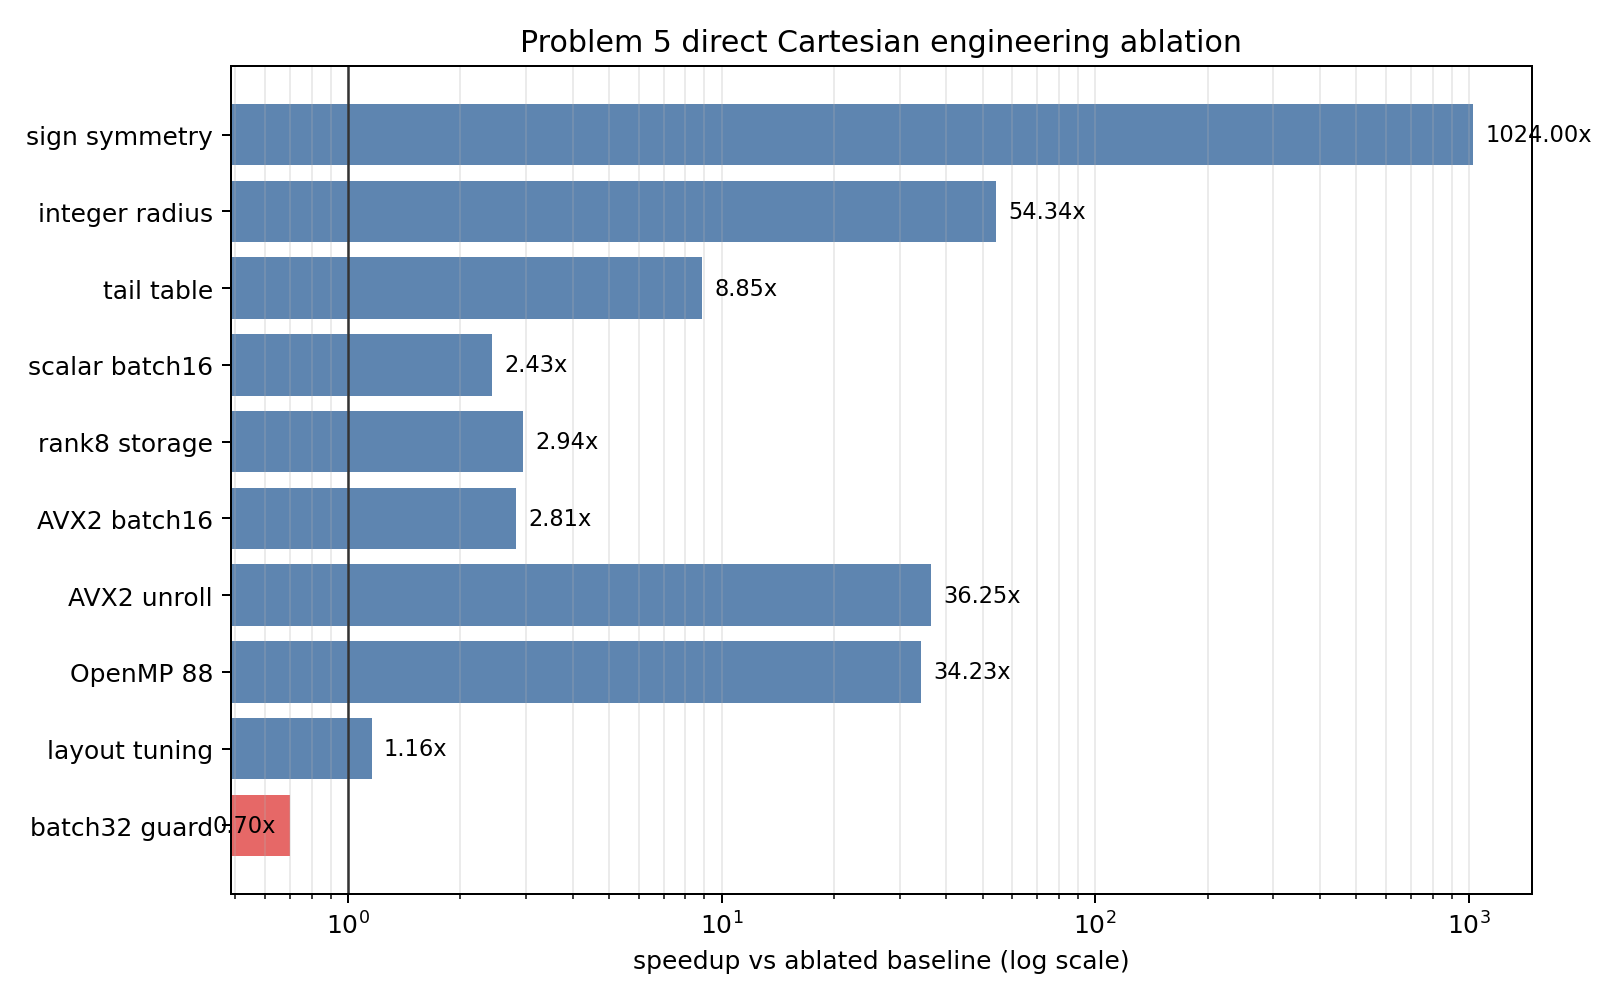
\includegraphics[width=0.96\linewidth]{../../../scripts/problem5_direct_cartesian/results/q23456_engineering_ablation_speedups.png}
  \caption{Problem 5 direct Cartesian 工程优化消融测试。横轴为相对去除该优化后的倍率，使用对数坐标；红色条表示 batch=32 的负收益检查。}
\end{figure}

上表除符号对称性需要按 \(2^n\) 换算 inside count 外，其余消融项的 inside count 原值均一致；因此这些测试比较的是等价 direct Cartesian 枚举实现的速度差异，而不是改变积分公式。符号对称性一行给出的是点数压缩倍率；它是题目积分区域的偶对称性，按 \(2^n\) 换算后不改变体积估计。layout 一行引用的是保存下来的 repeat-check 记录，说明参数需要实测筛选；同时 batch=32 的负收益说明并不是展开越多越好。最终 \(n=27,\ldots,30\) 的 direct run 在同一 strict rank8/AVX2/OpenMP 路径上达到 \(2.718\)--\(3.024\times10^{12}\) points/s，其中 \(n=30\) 的 tail 构造时间为 \(0.071\,\mathrm{s}\)，计数时间为 \(6681.206\,\mathrm{s}\)，主要瓶颈确实位于内层比较。

需要区分的是，代码中曾保留过 bitset storage 作为内部速度探索，但最终结果不使用该路径。bitset 会把 tail 比较进一步折叠成预构造集合的 popcount，虽然数值上可以等价，但从作业要求看有被解释为额外计数算子的风险；因此报告和最终表只采用 rank8 strict comparison 路线。

由于不同混合网格的相位误差差别很大，本题还使用了预测脚本来筛选超参数。预测机制不是随机抽样，也不是用经验曲线外推体积，而是对候选中点网格做精确有限网格误差分析。设候选参数只由各分辨率轴数
\[
\mathbf c=(c_2,c_3,c_4,c_5,c_6),\qquad \sum_{q=2}^6 c_q=n
\]
决定。由于积分区域和中点公式都对坐标置换不变，坐标轴的具体排列不影响候选误差；真正需要筛选的是这些计数
\(c_q\)。对一个分辨率为 \(q\) 的坐标轴，整数化后的单轴平方贡献为
\[
a_{q,k}=\left((2k+1)\frac{60}{q}\right)^2,\qquad k=0,\ldots,q-1.
\]
于是候选网格的整数半径平方分布可以写成生成函数
\[
F_{\mathbf c}(z)=
\prod_{q=2}^6
\left(\sum_{k=0}^{q-1}z^{a_{q,k}}\right)^{c_q}.
\]
其中 \(\left[z^s\right]F_{\mathbf c}(z)\) 正是第一卦限中整数半径平方等于 \(s\) 的中点个数，因此该候选的精确球内点数为
\[
C_{\mathrm{coeff}}(\mathbf c)=
\sum_{s\le 120^2}\left[z^s\right]F_{\mathbf c}(z).
\]
脚本实现时只保留 \(s\le120^2\) 的系数分布并做卷积更新；这是一种系数计数器。若把它直接作为最终体积结果，会偏离本题要求的逐点 direct Cartesian 枚举，所以本文只把它用于参数选择。

有了 \(C_{\mathrm{coeff}}(\mathbf c)\) 后，候选中点公式本身的体积估计为
\[
\widehat V_{\mathrm{coeff}}(\mathbf c)
=2^n\frac{C_{\mathrm{coeff}}(\mathbf c)}{\prod_{q=2}^6 q^{c_q}}.
\]
再用题面给出的参考公式
\[
V_{\mathrm{ref}}(n)=\frac{\pi^{n/2}}{\Gamma(n/2+1)}
\]
计算候选误差
\[
\varepsilon_{\mathrm{pred}}(\mathbf c)
=\left|\frac{\widehat V_{\mathrm{coeff}}(\mathbf c)-V_{\mathrm{ref}}(n)}
{V_{\mathrm{ref}}(n)}\right|.
\]
这就是本题筛参时所说的“预测误差”：它对候选网格是精确的，不含 Monte Carlo 噪声；但它只服务于“是否值得启动 strict direct run”的决策。运行时间则用
\[
T_{\mathrm{est}}(\mathbf c)=
\frac{\prod_{q=2}^6 q^{c_q}}{R_{\mathrm{strict}}}
\]
估计，其中 \(R_{\mathrm{strict}}\) 取自已经实测的 strict kernel 吞吐量。因此，预测脚本属于候选网格选择阶段；最终表格中的体积估计仍只使用 strict direct kernel 实际输出的 inside count。

实际筛选流程如下：先生成含 \(q=2\) 的 \(q=2,3,4,5,6\) 混合候选，并用点数比例、粗糙度指标和最小半径平方等条件去掉明显不合适的网格；然后对剩余候选计算
\(\varepsilon_{\mathrm{pred}}\) 和 \(T_{\mathrm{est}}\)；最后在
\(\varepsilon_{\mathrm{pred}}\le2\%\) 的候选中选择
\(\prod q^{c_q}\) 最小者。使用 \(2\%\) 而不是题目要求的 \(10\%\) 是为了给后续高维 direct 运行留出余量，并减少相位误差偶然性的风险。

这一筛选并不是手工试几个参数。当前记录中，\(n=27,28,29,30\) 分别检查了
\(2593,2845,3035,3281\) 个候选；其中预测相对误差低于 \(10\%\) 的候选分别为
\(388,299,228,161\) 个，低于 \(2\%\) 的候选分别为
\(45,37,28,25\) 个。也就是说，最终四个 direct run 是从数千个候选中按统一规则筛出的低点数候选，而不是事后根据 direct 结果反向挑选。

\begin{table}[H]
  \centering
  \small
  \setlength{\tabcolsep}{3pt}
  \begin{tabular}{r r r l r r r}
    \toprule
    \(n\) & 候选数 & \(<2\%\) 候选 & 选中网格 & \(C_{\mathrm{pred}}/C_{\mathrm{direct}}\) & 预测误差 & direct 时间 \\
    \midrule
    27 & 2593 & 45 & \(2^1 3^{16}4^7 6^3\) & \(516/516\) & \(1.990582\times10^{-2}\) & \(0.0280\,\mathrm{h}\) \\
    28 & 2845 & 37 & \(2^1 3^{16}4^7 5^2 6^2\) & \(487/487\) & \(1.588363\times10^{-2}\) & \(0.1272\,\mathrm{h}\) \\
    29 & 3035 & 28 & \(2^1 3^{14}4^{12}6^2\) & \(529/529\) & \(1.797700\times10^{-2}\) & \(0.5746\,\mathrm{h}\) \\
    30 & 3281 & 25 & \(2^1 3^{19}4^1 5^9\) & \(375/375\) & \(1.171641\times10^{-2}\) & \(1.8559\,\mathrm{h}\) \\
    \bottomrule
  \end{tabular}
\end{table}

表中 \(C_{\mathrm{pred}}/C_{\mathrm{direct}}\) 的一致性说明，预测脚本确实数的是同一套中点网格；但最终作业答案仍以后续 strict direct Cartesian 枚举得到的 inside count 和体积估计为准。预测脚本的作用是把高维参数选择从盲跑变成可控筛选：先用精确候选误差和时间估计排除大部分候选，再把少数满足阈值且点数最低的网格交给 direct kernel 实际计算。

\subsubsection{问题答案}\label{ux95eeux9898ux7b54ux6848-10}

\noindent\begin{minipage}{\linewidth}
\raggedright
核心脚本目录为 \textnormal{scripts/problem5\_direct\_cartesian/}。
\end{minipage}

\begin{table}[H]
  \centering
  \small
  \setlength{\tabcolsep}{4pt}
  \begin{tabular}{>{\raggedright\arraybackslash}p{0.60\linewidth}>{\raggedright\arraybackslash}p{0.30\linewidth}}
    \toprule
    脚本 & 用途 \\
    \midrule
    \shortstack[l]{\textnormal{direct\_tensor\_midpoint\_orthant\_mixed\_q26\_}\\\textnormal{tile\_batch\_avx2.c}} & 最终 strict direct C kernel \\
    \textnormal{run\_q23456\_coefficient\_search.py} & 筛选候选网格 \\
    \textnormal{run\_q23456\_select\_under30\_results.py} & 选出 \(n=27,\ldots,30\) 的紧凑候选 \\
    \textnormal{run\_q23456\_selected\_under30\_direct.py} & 执行 strict direct 直算 \\
    \textnormal{run\_q23456\_strict\_layout\_optimization\_tests.py} & 比较 tail 维数、chunk、轴顺序和 batch 布局 \\
    \textnormal{run\_q23456\_strict\_layout\_repeat\_checks.py} & 对低风险 layout 选择做重复测量 \\
    \textnormal{run\_q23456\_ablation\_tests.py} & 运行工程优化消融测试并生成图表 \\
    \textnormal{direct\_tensor\_midpoint\_ablation\_kernel.c} & 提供消融测试的 scalar proxy kernel \\
    \bottomrule
  \end{tabular}
\end{table}

本题的结果文件也分成“筛选、直算、工程验证”三类。为避免长文件名把表格撑得过宽，下面只按用途列出核心记录：

\begin{table}[H]
  \centering
  \footnotesize
  \setlength{\tabcolsep}{5pt}
  \renewcommand{\arraystretch}{1.22}
  \begin{tabular}{>{\raggedright\arraybackslash}p{0.16\linewidth}>{\raggedright\arraybackslash}p{0.74\linewidth}}
    \toprule
    类别 & 核心记录与作用 \\
    \midrule
    候选筛选 &
    \textnormal{q23456\_coefficient\_search\_predictions.csv} 记录 \(n=27,\ldots,31\) 的候选筛选结果，共 \(15282\) 条候选记录，只用于选择候选参数。 \\
    候选固化 &
    \textnormal{q23456\_selected\_under30\_results.csv} 固化 \(n=27,\ldots,30\) 的最终候选规则：在预测误差不超过 \(2\%\) 的候选中取点数最小者。 \\
    直接计算 &
    \textnormal{q23456\_selected\_under30\_direct\_results.csv} 保存 strict direct kernel 的实际 inside count、体积估计、计数时间和吞吐量。 \\
    layout 验证 &
    \textnormal{q23456\_strict\_layout\_optimization\_benchmark.csv} 和
    \textnormal{q23456\_strict\_layout\_repeat\_benchmark.csv} 记录单次基准和重复基准，用于排除一次性噪声并支持 \(n=31\) 时间估计。 \\
    工程消融 &
    \textnormal{q23456\_engineering\_ablation\_raw.csv} 和
    \textnormal{q23456\_engineering\_ablation\_summary.csv} 检查优化前后 inside count 是否保持一致，并量化每类优化的速度影响。 \\
    \bottomrule
  \end{tabular}
\end{table}

实际完成的 strict direct Cartesian 结果如下：

\begin{table}[H]
  \centering
  \small
  \setlength{\tabcolsep}{3pt}
  \renewcommand{\arraystretch}{1.12}
  \begin{tabular}{r >{\raggedright\arraybackslash}p{0.30\linewidth} r r r r}
    \toprule
    \(n\) & 网格模式 & 球内点数 & 估计体积 & 相对误差 & 计数时间 \\
    \midrule
    27 & \(2^1 3^{16}4^7 5^0 6^3\) & 516 & \(2.2730858\times10^{-4}\) & \(1.990582\times10^{-2}\) & \(100.7609\,\mathrm{s}\) \\
    28 & \(2^1 3^{16}4^7 5^2 6^2\) & 487 & \(1.0297607\times10^{-4}\) & \(1.588363\times10^{-2}\) & \(457.9538\,\mathrm{s}\) \\
    29 & \(2^1 3^{14}4^{12}5^0 6^2\) & 529 & \(4.9155893\times10^{-5}\) & \(1.797700\times10^{-2}\) & \(2068.7067\,\mathrm{s}\) \\
    30 & \(2^1 3^{19}4^1 5^9 6^0\) & 375 & \(2.2172123\times10^{-5}\) & \(1.171641\times10^{-2}\) & \(6681.2057\,\mathrm{s}\) \\
    \bottomrule
  \end{tabular}
\end{table}

其中 \(n=30\) 的第一卦限总点数为

\[
2^1 3^{19}4^1 5^9=18160335421875000,
\]

实际吞吐量为

\[
2.718122488\times 10^{12}\ \text{points/s}.
\]

所有 \(n=27,\ldots,30\) 结果的相对误差都低于 \(10\%\)，其中 \(n=28\) 与 \(n=30\) 均满足题目对高维计算的要求。参考体积仅在直算完成后用于误差核对，例如 \(n=30\) 的参考值为 \(2.1915353447830204\times10^{-5}\)，相对误差为 \(1.171641\times10^{-2}\)。

\subsubsection{分析}\label{ux5206ux6790-10}

这个方案能从 \(28\) 维推进到 \(30\) 维，核心原因有两个：第一，混合分辨率把第一卦限张量点数从均匀细网格的规模压到更低；第二，strict kernel 把每个张量点的判定代价压到接近内存连续扫描和向量比较的极限。最终运行时间可以用简单性能模型解释：
\[
T_{\mathrm{count}}\approx \frac{P(\mathbf q)}{R},\qquad
R\approx (2.7\text{--}3.0)\times10^{12}\ \text{points/s}.
\]
例如 \(n=30\) 时，如果直接使用均匀 \(q=4\) 中点张量，第一卦限需要
\[
4^{30}=1.152921504606846976\times10^{18}
\]
个点。按实际 \(n=30\) 吞吐量估算，计数时间约为 \(117.82\) 小时，即
\(4.91\) 天。最终选出的混合网格
\(2^1 3^{19}4^1 5^9 6^0\) 只需要
\[
1.8160335421875\times10^{16}
\]
个点，点数减少约 \(63.49\times\)，实测计数时间为 \(6681.21\,\mathrm{s}\)，即
\(1.856\) 小时。

\begin{table}[H]
  \centering
  \small
  \setlength{\tabcolsep}{4pt}
  \begin{tabular}{l r r r}
    \toprule
    \(n=30\) 网格 & 第一卦限点数 & 时间来源 & 计数时间 \\
    \midrule
    均匀 \(q=4\) & \(1.1529\times10^{18}\) & 按实测吞吐量估算 & \(117.82\,\mathrm{h}\) \\
    混合 \(2^1 3^{19}4^1 5^9\) & \(1.8160\times10^{16}\) & 实际 direct run & \(1.856\,\mathrm{h}\) \\
    \bottomrule
  \end{tabular}
\end{table}

混合分辨率中出现 \(q=2\) 或 \(q=3\) 并不意味着把高维问题粗暴降精度到低阶公式。它的含义是：在某些坐标轴上使用较粗的中点网格，换取 \(P(\mathbf q)\) 的指数级下降；同时在另一些坐标轴上使用 \(q=4,5,6\) 来调整边界相位。由于球指标函数的误差主要来自边界小盒，单纯增加所有坐标的 \(q\) 并不总是最高效；更有效的做法是在给定计算预算内选择相对误差可接受的混合相位。最终 \(n=27,\ldots,30\) 的相对误差均低于 \(2\%\)，明显满足 \(10\%\) 阈值。

工程消融表说明，最终速度不是某一个技巧单独带来的，而是多个低风险优化叠加后的结果。整数半径更新消除了每点 \(O(n)\) 浮点求和，tail 表复用把重复坐标生成移出内层循环，rank8 把主循环读带宽降到字节级，prefix batching 让同一段 tail 数据服务多个阈值，AVX2 展开把比较和计数做成宽向量指令，OpenMP 则把 prefix 空间分配给多核。由于这些消融项保持相同的体积估计（符号对称性按 \(2^n\) 换算，其余 inside count 原值一致），这些优化改变的是执行代价，而不是积分公式。

从工程角度看，这组尝试还提供了两个反面约束。第一，bitset storage 虽然在程序中作为探索路径存在，但它会把 tail 阈值比较变成预构造集合的 popcount，报告中没有把它作为最终结果路径。第二，更大的 batch 不一定更快；重复测试中 \texttt{batch\_prefixes}=32 的速度只有 batch=16 的约 \(0.70\times\)。因此最终路线保留的是“仍逐项比较、但把比较做得更便宜”的优化，而不是把计数问题改写成另一种压缩算子。

该方法仍然没有消除指数墙。对于固定误差阈值，维数继续增加时
\(P(\mathbf q)\) 仍会快速上升；layout 调参只能把常数因子继续压低，不能把
\(\Theta(P(\mathbf q))\) 改成多项式时间。额外测试表明，把
\texttt{batch\_prefixes} 从 \(16\) 增加到 \(32\) 在本机上反而变慢，原因很可能是寄存器压力和溢出增加。因此最终 direct 路线仍采用 \texttt{batch\_prefixes=16}。对 \(n=31\) 的严格 direct 估计仍约为 \(9\) 到 \(10\) 小时：最便宜的 \(10\%\) 内候选约 \(8.336\) 小时，预测误差低于 \(2\%\) 的候选约 \(9.656\) 小时。

\subsection{Problem 5(b)：维数变化与方法边界}\label{problem-5b}

\scriptlink{problem5_direct_cartesian/}

\subsubsection{待求问题}\label{ux5f85ux6c42ux95eeux9898-11}

在屏幕输出结果，并说明超球体积随维数变化的趋势。

\subsubsection{解决方式}\label{ux89e3ux51b3ux65b9ux5f0f-11}

维数变化的定性趋势用题面给出的解析公式作参考；该公式不参与 direct 结果生成，只用于解释体积随维数的整体变化和计算相对误差。直接中点张量积分则用于 \(n=27,\ldots,30\) 的实际高维数值验证。为了让趋势更直观，脚本额外绘制 \(n=0,\ldots,35\) 的线性坐标曲线和 \(n=1,\ldots,100\) 的对数坐标曲线，并在图中叠加已经实际完成的 \(n=27,\ldots,30\) direct 点。

\subsubsection{问题答案}\label{ux95eeux9898ux7b54ux6848-11}

单位球体积先随维数增加而增大，在低维达到峰值后迅速下降。对本题直接数值实验而言，已经实际完成到 \(n=30\)，且所有高维 direct 结果均在 \(10\%\) 相对误差以内。继续到 \(n=31\) 在本机上仍可行，但需要接近半天的 CPU 时间；若继续增加维数，指数墙仍会重新成为主要限制。

\begin{figure}[H]
  \centering
  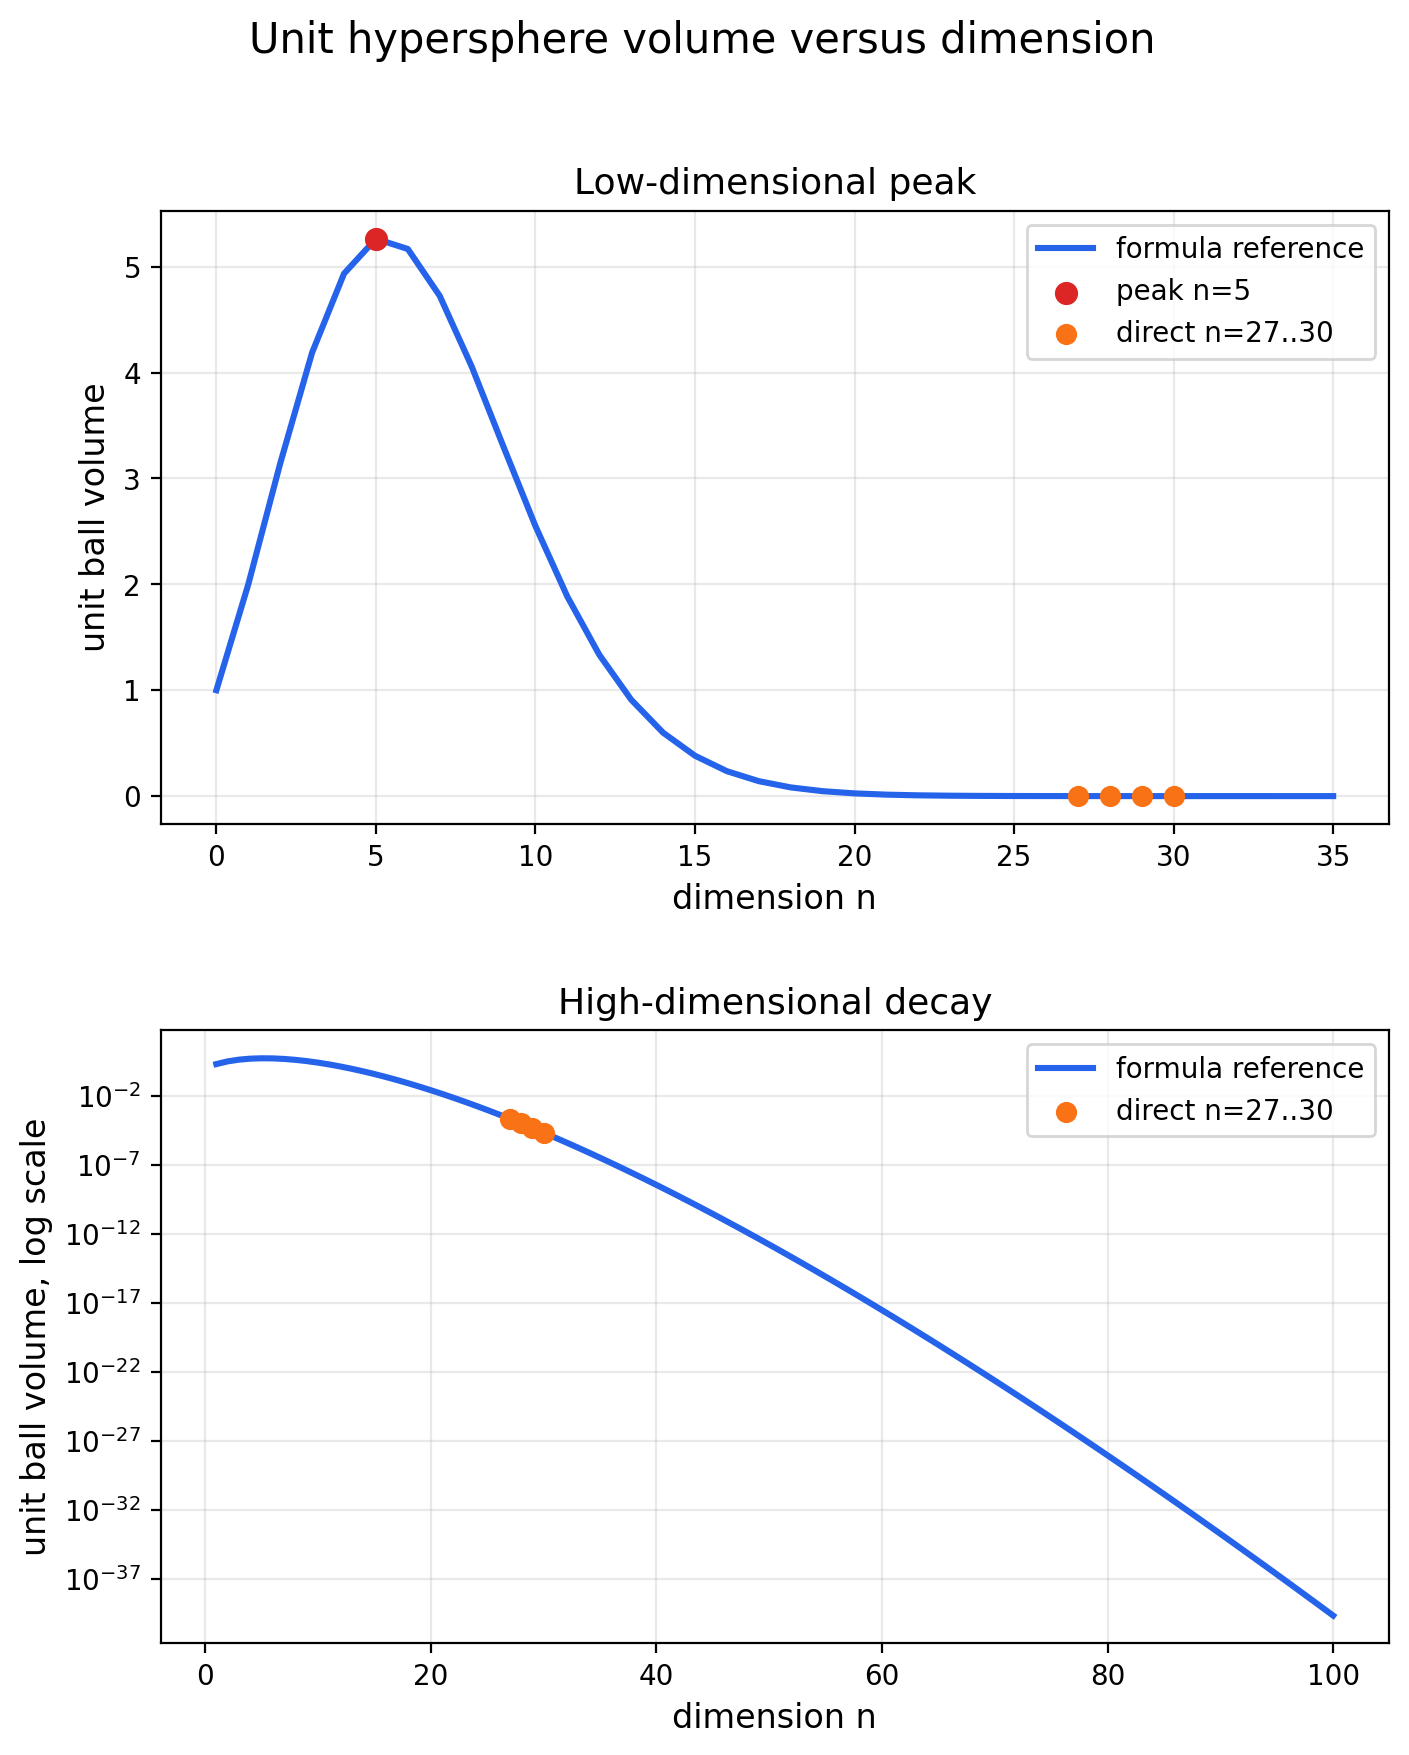
\includegraphics[width=0.96\linewidth]{../../../result/problem5_volume_trend_formula.png}
  \caption{单位超球体积随维数变化的趋势。上图显示低维峰值，下图用对数坐标显示高维快速衰减；橙色点为本题实际 direct Cartesian 计算得到的 \(n=27,\ldots,30\) 结果。}
\end{figure}

从图中可以直接看到，单位半径超球体积在 \(n=5\) 附近达到最大值 \(V_5\approx5.263789\)，随后随维数增加迅速下降。线性坐标下 \(n>20\) 的体积已经贴近横轴，因此下方对数坐标更适合观察 \(n=30\) 以后继续下降的趋势。

\subsubsection{分析}\label{ux5206ux6790-11}

从题面参考公式结合 Stirling 公式可得

\[
\Gamma\!\left(\frac{n}{2}+1\right)
\sim \sqrt{\pi n}\left(\frac{n}{2e}\right)^{n/2},
\qquad n\to\infty,
\]

于是

\[
V_n=\frac{\pi^{n/2}}{\Gamma(n/2+1)}
\sim
\frac{1}{\sqrt{\pi n}}
\left(\frac{2\pi e}{n}\right)^{n/2}.
\]

当 \(n\) 足够大时，\((2\pi e/n)^{n/2}\) 快速趋于 \(0\)，因此单位半径超球体积最终趋于 \(0\)。这也解释了为什么高维体积虽然可以用题面公式很快写出，但若坚持 direct Cartesian tensor 积分，计算量仍随维数指数增长。当前方法的意义不在于消除指数墙，而是在不使用随机法、闭式公式或体积递推作为结果路径的前提下，通过混合分辨率和工程优化把实际 direct 计算推进到 \(30\) 维。

\end{document}
